\section{Introduction}


Spoken words create analog signals that are processed by the brain in real time. That is, as spoken word unfolds, a collection of candidate words are considered until the target word is recognized \citep{MarslenWilson1987}. The degree to which a particular candidate word is being considered is known as activation. An important part of this process involves not only correctly identifying the word but also eliminating competitors. For example, we might consider a discrete unfolding of the word ``elephant" as ``el-e-phant". At the onset of ``el", a listener may activate a cohort of potential resolutions such as ``elephant", ``electricity", or ``elder", all of which may be considered competitors. With the subsequent ``el-e", words consistent with the received signal, such as ``elephant" and ``electricity" remain active competitors, while incompatible words, such as ``elder", are eliminated. Such is a rough description of this process, continuing until the ambiguity is resolved and a single word remains.


Our interest is in measuring the degree of activation of a target word, relative to competitors. Activation, however, is not measured directly, and we instead rely on what can be observed with physiological behavior. Although there are a number of relevant indices of lexical activation \citep{Spivey2005}, we concern ourselves here with eye tracking data collected in the context of the Visual World Paradigm (VWP) \citep{tanenhaus1995integration}, an experimental model in which a participant's eye movements are tracked as they respond to spoken language. Recently, however, researchers have begun to reexamine some of the underlying assumptions associated with the VWP, calling into question the validity or interpretation of current methods (\citep{Magnuson2019}, \citep{mcmurray2022m}). We present here a brief history of word recognition in the context of the VWP, along with an examination of contemporary concerns. In response, we then propose a new generative model for understanding eye mechanics, accompanied by an alternative method for relating eye-tracking data to lexical activation. We follow this with a series of simulations, both in the context of recovering the trajectory of eye mechanics for individual subjects, as well as for identifying differences in trajectories between groups of individuals. Finally, we demonstrate the performance of our model with an application to data collected in prior studies. 


\paragraph{Visual World Paradigm} The Visual World Paradigm  was first introduced in 1995, marking the initial link between the mental processes associated with language comprehension and eye movements \citep{tanenhaus1995integration}. A typical experiment in the VWP involves situating a subject in front of a ``visual world", commonly a computer screen today, and asking them to identify and select an object corresponding to a spoken word. The initiation of eye movements and subsequent fixations are recorded as this process unfolds, with the location of the participants' eyes serving as a proxy for which words or images are being considered. This association was first demonstrated by comparing how the mean time to initiate an eye movement to the correct object was mediated by the presence of phonological competitors (``candy" and ``candle", sharing auditory signal at word onset) and situations containing syntactic ambiguity (``Put the apple on the towel in the box" and ``Put the apple \textit{that's} on the towel in the box" in ambiguous scenarios with one or more apples). It is by comparing the trajectory of these mechanics across trials in the presence of auditory or semantic competitors that researchers have used the VWP in their investigation of spoken word recognition. For a review of the Visual World Paradigm and its applications, see \citet{Huettig2011}, \citet{salverda2017visual}.




\paragraph{Proportion of fixation} The interactive activation model of word recognition was first introduced in \citet{McClelland1981}, positing that word recognition takes place in a system with multiple interacting hierarchies of processing, including those made up of features, phonemes, and words. This model was later instantiated as a computer model known as TRACE \citep{elman1985speech}. Briefly, TRACE is structured as a hierarchical network model in which input is fed into the system (typically as a string of phonemes) with potential resolutions (here, words) being represented as nodes. The TRACE model processes this input over time and in parallel, with activation incrementally cascading from features (voicing, aspiration, etc.,) to phonemes to words. Multiple words can be activated at once, graded by consistency of the word with the received signal. Finally, the TRACE model exhibits competition whereby the activation of a particular word functions to inhibit its competitors. This entire process continues as input is received until a single word is most active. An example of this is demonstrated in Figure~\ref{fig:trace_plot} using the current implementation of TRACE, jTRACE \citep{Strauss2007}, in which the word ``party" was provided as input as a string of phonetic characters. Figure~\ref{fig:trace_plot} shows the activation of the target word, along with a number of competitors.

\begin{figure}[H]
\centering
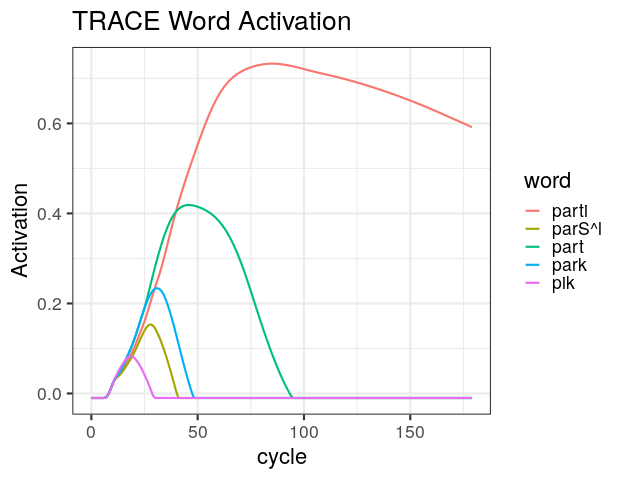
\includegraphics[scale=1]{trace_plot}
\caption{TRACE activation of the word ``party", with competitors}
\label{fig:trace_plot}
\end{figure}



It was against simulated TRACE data that \citet{allopenna1998tracking} found a tractable way of analyzing eye-tracking data collected in the VWP.  During each trial, the location of an eye fixation was recorded at intervals of 33ms and was marked as either a $0$ or $1$ as an indicator of whether or not the subject was fixated on the referent or not. By taking the average of fixations towards a referent at each time point, Allopenna was able to create a ``fixation proportion" curve that largely reflected the shape and competitive dynamics of word activation suggested by TRACE, both for the target object as well as for competitors, giving researchers a method to both visualize and quantify the time course of lexical activation. This also provided an empirical grounding for an explicit linking hypothesis, relating activation to eye mechanics  (emphasis added):

\begin{quote}
We made the general assumption that the probability of initiating an eye movement to fixate on a target object $o$ at time $t$ is a direct function of the probability that $o$ is the target given the speech input and where the probability of fixating $o$ is determined by the activation level of its lexical entry relative to the activation of other potential targets. [...] Note that this hypothesis does \emph{not} require stronger and less defensible assumptions about the relationship between eye  movements and attention. For example, we are not committed to the assumption that scan patterns in and of themselves reveal underlying cognitive processes. \citep{allopenna1998tracking}
\end{quote}

The utility in this linking hypothesis comes from its simplicity, asserting only that the probability of fixating an object increases as the likelihood it has been referred to also increases. This is in contrast to a number of more involved linking hypotheses presented in \citet{Magnuson2019}.


\begin{figure}[H]
\centering
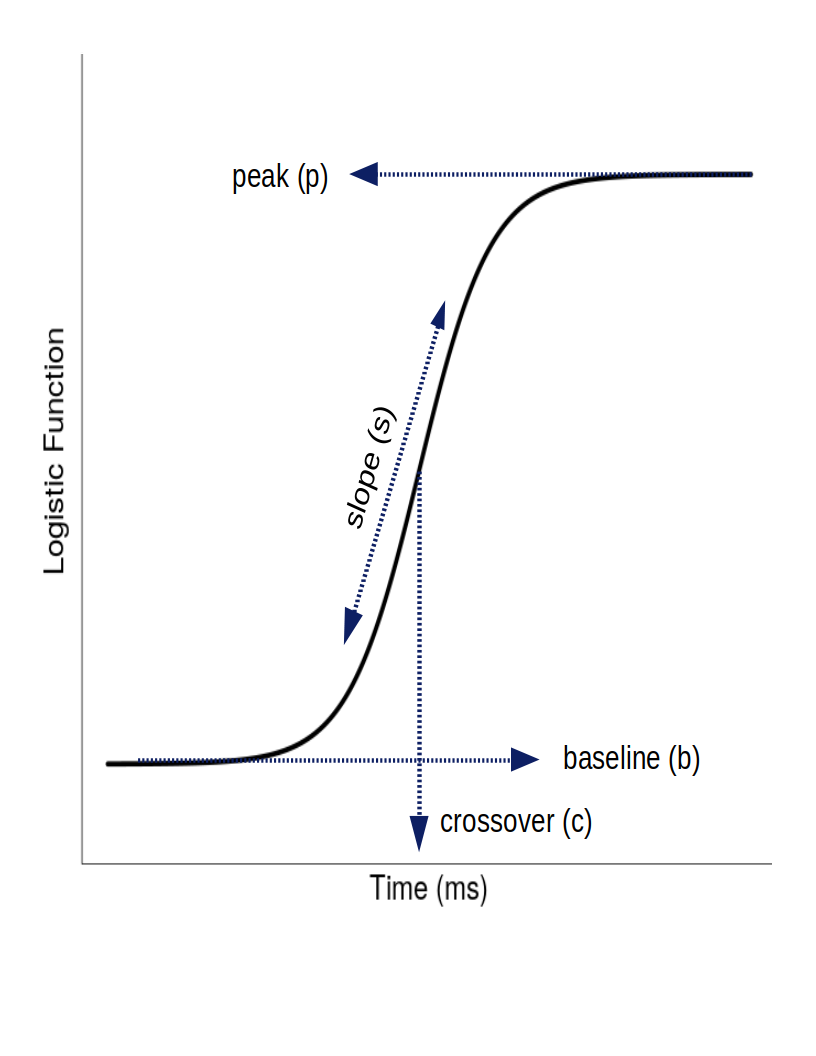
\includegraphics[scale=0.4]{logistic_label.png}
\caption{An illustration of the four-parameter logistic (Equation~\ref{eq:logistic1}) and its associated parameters, introduced as a parametric function for fixations to target objects}
\label{fig:logistic_definition}
\end{figure}

\paragraph{Parametric Methods and Individual Curves} While many studies have addressed qualitative aspects of word recognition such as feedback \citep{Magnuson2003}, or priming \citep{luce1998delayed}, few had offered consideration to individual differences in activation. A first attempt was provided by \citet{Mirman2008} using mixed effects models to capture subject-specific effects by fitting observed data to polynomial functions in time. While this addressed the problem of capturing individual differences, it was burdened by the fact that polynomials are often a poor fit for VWP data, often requiring a high degree to be appropriately fit, resulting in potentially poor asymptotic behavior. Further, polynomial coefficients are often unable to be intuitively mapped onto clinically relevant properties of the functions they are intended to emulate. This was the position taken by \citet{mcmurray2010individual}, who first introduced non-linear functions to the observed data, equipped with readily interpretable and clinically relevant properties. This includes the four parameter logistic function provided in Equation~\ref{eq:logistic1} as well as the asymmetric Gaussian function given in Equation~\ref{eq:dg2}. Outside of serving to address psycholinguistic concerns relating to individual differences in word recognition, this advancement has been critical in shaping current statistical models used in the context of the VWP. The specification of subject-specific parameters itself implies a distribution of parameters within an experimental group, serving as an impetus for investigating group differences in word activation through the use of bootstrapped differences in time series \citep{oleson2017detecting} and the subsequent development of the \xt{bdots} software in R for analyzing such differences \citep{seedorff2018bdots}.



\section{Analysis with VWP Data}

We now shift focus to the physiological mechanics of eye movements in the context of the Visual World Paradigm, including a mathematical description of how these mechanics relate to the proportion of fixation method first introduced by \citet{allopenna1998tracking}.  




\subsection{Anatomy of Eye Mechanics}

While a number of experimental methods are used as real-time indices of lexical access \citep{Spivey2005}, we concern ourselves here with the use of eye tracking, given that ``eye movements to objects in the workspace are closely time-locked to referring expressions in the unfolding speech stream, providing a sensitive and non-disruptive measure of spoken language comprehension during continuous speech \citep{allopenna1998tracking}." This process in its entirety is made up of several interrelated components, including activation and the visual-motor system, oculomotor delay, and mechanics of eye movement itself. We briefly introduce each of these components in turn, while providing a visual summary in Figure~\ref{fig:whats_in_a_look}.

\begin{figure}[H]
\centering
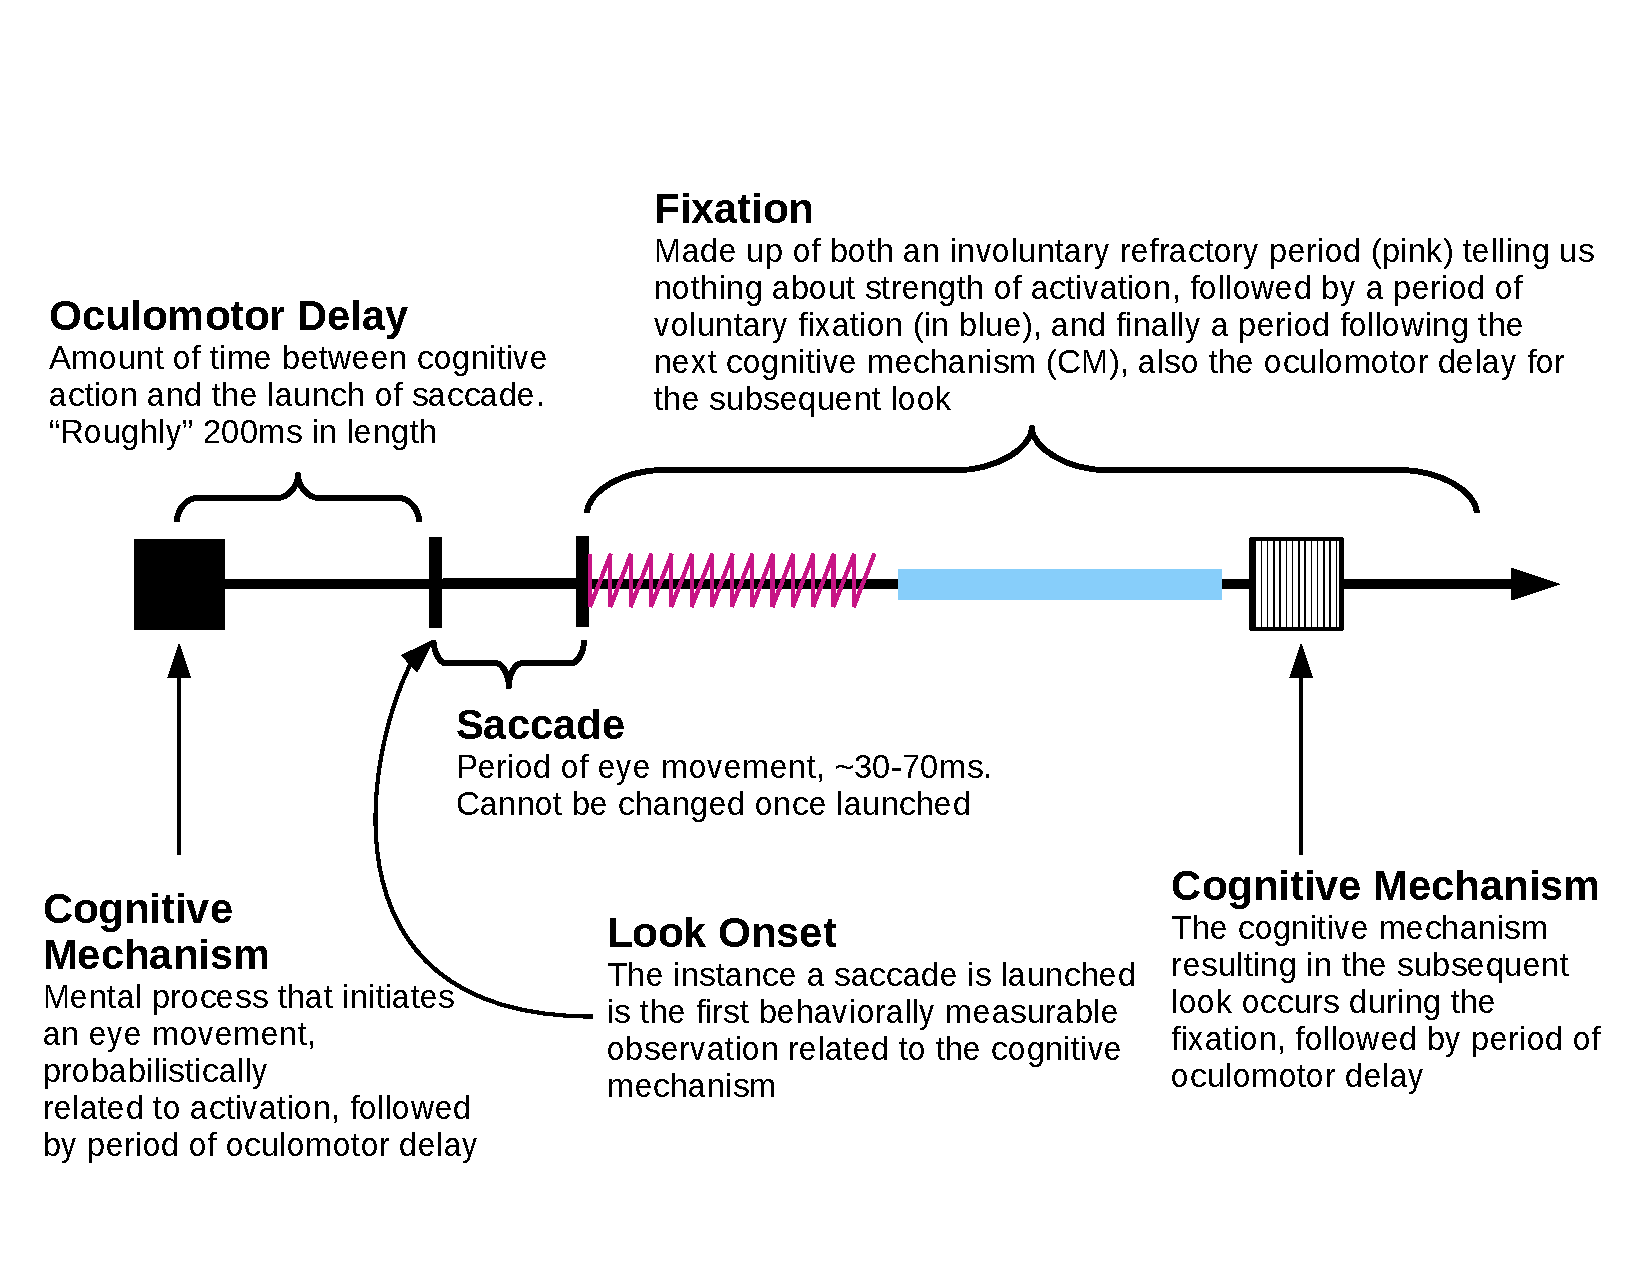
\includegraphics[scale=0.5]{what_is_a_look.pdf}
\caption{Anatomy of a look} 
\label{fig:whats_in_a_look}
\end{figure}

\subsubsection{Saccades and Fixation}

Rather than acting in a continuous sweeping motion as our perceived vision might suggest, our eyes themselves move about in a series of short, ballistic movements, followed by brief periods of stagnation. These periods of movement and stagnation, respectively, are the saccades and fixations. 

Saccades are short, ballistic movements lasting between 20ms-60ms, during which time we are effectively blind. Once in motion, saccades are unable to change trajectory from their intended destination. Following this movement is a period known as a fixation, itself made up of a necessary refraction period (during which time the eye is incapable of movement) followed by a period of voluntary fixation which may include planning time for deciding the destination of the next eye movement. Additionally, the duration of fixations are typically longer and more variable. It will be convenient to follow previous convention and consider a saccade followed by its adjacent fixation as a single concept called a ``look" \citep{mcmurray2002look}. We take particular care here to note that the beginning of a look, or ``look onset", starts the instance that a previous look ends or, said another way, the instant an eye movement is launched. 

The mechanical aspects of eye movements are not themselves what we are interested in. Rather, they serve as an index of the underlying cognitive process, lexical activation, which we discuss next.

\subsubsection{Activation and Visual-Motor system}

The concept of activation, as it relates to the discussion here, arises from the metaphor in which word perception is made up of a network made up of hierarchical levels (letter, phoneme, word, etc.,) acting as an interactive process unfolding in time \citep{McClelland1981}. Under this \textit{interactive activation model}, greater activation is associated with a greater excitatory action for a network node (specifically here a word) resulting from consistency with the received auditory signal. The interactive activation model allows for both excitatory and inhibiting activations, resulting in the ``competing" activation curves between candidate resolutions as the auditory signal unfolds. A theoretical example of activation is given in Figure~\ref{fig:trace_plot}.

Eye movements themselves are not a direct read-out of activation, and instead are downstream of a much larger process that also involves the visual-motor system, including general stimulus processing and environment scanning \citep{Salthouse1980}. It is this peripheral system, in conjunction with lexical activation, that leads to the \textit{probabilistic} association of activation and fixations. Any proposed relation of each of these in detail to saccades and fixations is known as a \textit{linking hypothesis} tying the observed to the theoretical \citep{Magnuson2019}. 

For our purposes here, we take no stronger a position than acknowledging the interplay between these processes and acknowledging their culmination as a ``cognitive mechanism" (CM) that ultimately is responsible for initiating the launching of a saccade, a mechanism itself that is probabilistically related to activation.



\subsubsection{Oculomotor Delay}

In between the cognitive mechanism that initiates the decision to launch an eye movement and the movement itself is a period known as oculomotor delay. It is typically estimated to take around 200ms to plan and launch an eye movement \citep{viviani1990time}, and this is usually accounted for by subtracting 200ms from any observed behavior. As oculomotor delay is only ``roughly" estimated to be around 200ms, we suggest that accounting for randomness will be critical in correctly recovering the cognitive mechanism of interest or at very least in identifying possible sources of bias or error. 





\subsection{Proportion of Fixation Method}


We now consider how the aforementioned mechanics relate to the Visual World Paradigm. In a typical implementation of the VWP, a participant is asked to complete a series of trials during each of which they are presented with a number of competing images on screen (typically four). A verbal cue is given, and the participants are asked to select the image corresponding to the spoken word. All the while, participants are wearing (generally) a head-mounted eye tracking system recording where on screen they were fixated. 

An individual trial of the VWP may be short, lasting anywhere from 1000ms to 2500ms before the correct image is selected. Prior to selecting the correct image, the participant's eyes scan the environment considering images as potential candidates to the spoken word. As this process unfolds, a snapshot of the eye is taken at a series of discrete steps (typically every 4ms) indicating where on the screen the participant is fixated. A single trial of the VWP typically contains no more than four to eight total ``looks" before the correct image is clicked, resulting in a paucity of data in any given trial.

To be clear, eye trackers themselves only record $x$ and $y$ coordinates of the eye at any given time, and it is only after the fact that ``psycho-physical" attributes are mapped onto the data (saccades, fixations, blinks, etc.,). We adopt the strategy of prior work in discussing eye tracking data in terms of their physiological mapping, as this will be crucial in constructing a physiologically relevant understanding of the problem at hand \citep{mcmurray2002look}.

\begin{figure}[H]
\centering
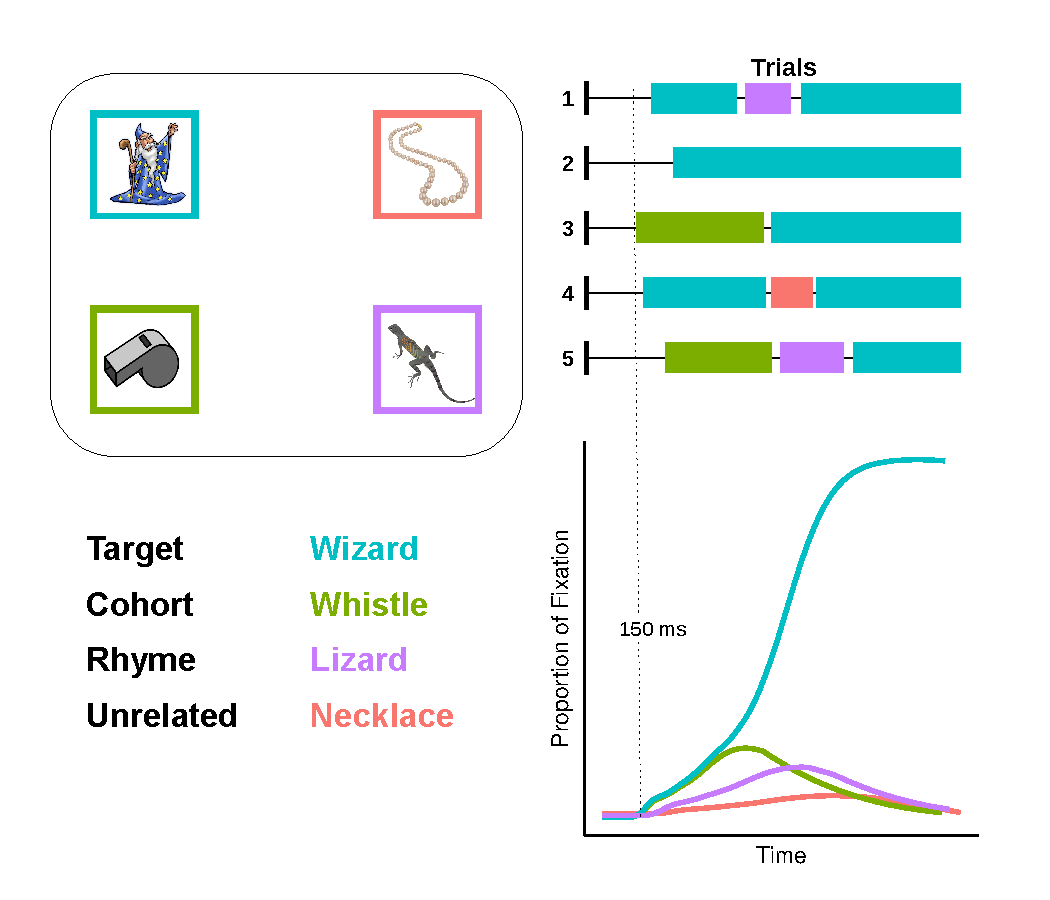
\includegraphics[scale=0.7]{collin_diagram_full.pdf}
\caption{Trials in the Visual World Paradigm}
\label{fig:collin_diagram_full}
\end{figure}


To create a visual summary of this process aggregated over all of the trials, a la Allopena, a ``proportion of fixations" curve is created, aggregating at each discrete time point the average of indicators of whether or not a participant is fixated on a particular image. A resulting curve is created for each of the competing categories (target, cohort, rhyme, unrelated), creating an empirical estimate of the activation curve, $f(t|\theta)$. See Figure~\ref{fig:collin_diagram_full}. For any subject $i = 1, \dots, n$, across times $t = 0, \dots, T$ and trials $j = 1, \dots, J$, a construction  of this curves can be expressed as:


\begin{equation}\label{eq:sum_proportions}
y_{it} = \frac1J \sum_{j=1}^J z_{ijt}
\end{equation}
where $z_{ijt}$ is an indicator $\{0, 1\}$  towards a particular object in trial $j$ at time $t$. Following the contributions of \citet{mcmurray2010individual}, we model the empirical curve given in Equation~\ref{eq:sum_proportions} with a parametric function $f(t|\theta)$, identifying subject-specific parameters $\theta_i$ which describe clinically relevant attributes of the curve, 

\begin{equation}\label{eq:empir_to_activation}
f(t | \theta_i) \equiv y_{it}.
\end{equation}

The recovery of subject-specific parameters occurs by subjecting the observed data to a simple loss function, 

\begin{equation}\label{eq:prop_loss}
\hat{\theta} = \argmin_{\theta} \mathcal{L}(f_{\theta}, y).
\end{equation}

As mentioned previously, fixations to the Target in a VWP experiment are often modeled with the four parameter logistic function (Figure~\ref{fig:logistic_definition}):

\begin{equation} \label{eq:logistic1}
f(t|\theta) = \frac{p-b}{1 + \exp \left(\frac{4s}{\text{p}-b} (x - t) \right)} + b.
\end{equation}

Similarly, a six parameter asymmetric Gaussian function \cn{(Figure updating figures)}, often used for fixations to competitors, is given as

\begin{equation} \label{eq:dg2}
f(t|\theta) = \begin{cases}
\exp \left( \frac{(t - \mu)^2}{-2\sigma_1^2} \right) (p - b_1) + b_1 \quad \text{if } t \leq \mu \\
\exp \left( \frac{(t - \mu)^2}{-2\sigma_2^2} \right) (p - b_2) + b_2 \quad \text{if } t > \mu
\end{cases}
\end{equation}


In a typical VWP study, the collection of subject-specific curves is used to estimate temporal characteristics of a larger group, for example, identifying how the process of lexical activation differentiates itself between groups of typically developed children and those with specific cognitive disabilities. As such, it is critical that data collected in the VWP be able to not only accurately reflect relevant characteristics of individual subjects, but also that these characteristics are preserved in the aggregate such that meaningful differences can be correctly identified. This is facilitated by having accurate and tractable models relating lexical activation to physiologically observable data. 

To this end, and in light of the discussion of the mechanics presented here, we propose an alternative model linking data recorded in the VWP with lexical activation, centered around the cognitive mechanism initiating eye movements. We call this the look onset method, which we present in the next section.




\section{Look Onset Method}

\begin{figure}[H]
\centering
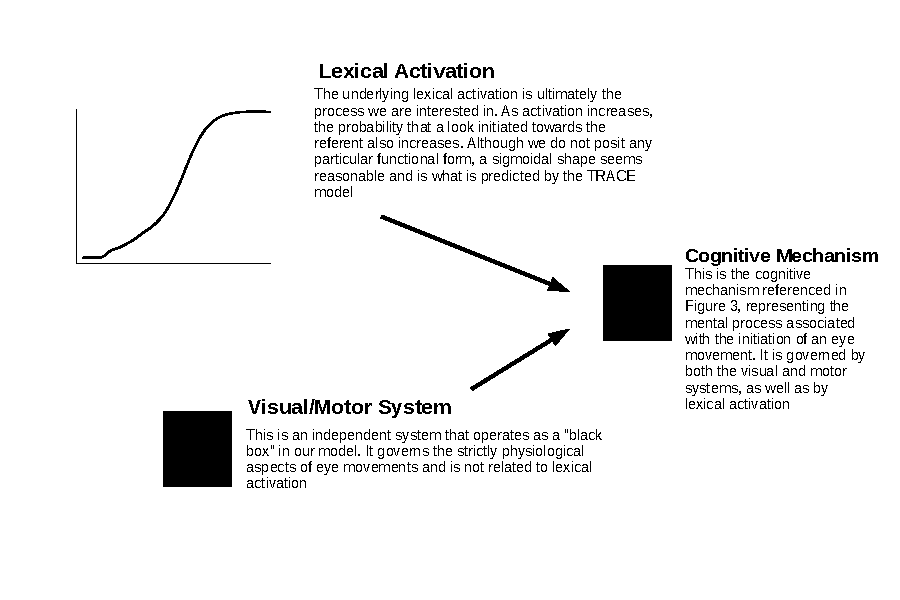
\includegraphics[scale=1]{black_box_system.pdf}
\caption{The cognitive mechanism that determines the destination of a look is a function of both lexical activation and the underlying visual/motor system}
\label{fig:black_box_model}
\end{figure}


In this section, we present a new method for utilizing data in the Visual World Paradigm in pursuit of the recovery of latent activation. From the physiologically grounded model presented in Figure~\ref{fig:whats_in_a_look}, we argue for delineating the several related but ultimately \emph{distinct} processes associated with eye mechanics. The primary of these, and the focus of the method we present here, is that of the cognitive mechanism responsible for initiating eye movements. Additionally, we consider the processes responsible for the duration of a fixation, as well as that governing oculomotor delay.

\subsection{Look Onset Method}

Outside of the implicit acknowledgement that the destination of saccadic eye movements are probabilistically related to lexical activation, we identify the cognitive mechanism initiating this movement as the first event downstream this cognitive process that culminates as a physiologically measurable phenomenon in the context of eye tracking data, despite the period of oculomotor delay separating this mechanism from the subsequent saccade. 

Nonetheless, in the context of a Target object in the VWP (or any other specific referent), we can frame this mechanism as a Bernoulli event whereby the probability of this event resulting in a fixation to the Target object is determined by the activation level of that particular referent. In the case of a Target object, for example, this probability increases concomitant with the amount of auditory stimulus received.

From this observation, we propose here what we call the \textit{look onset method}, which holds that the destination of a saccade launched at some time $t$, $s_t$, is probabilistically determined by its lexical activation at time $t$. Letting $f(t|\theta)$ denote the lexical activation to the Target at time $t$, for example, gives

\begin{equation}\label{eq:onset_distribution}
s_t \sim Bern \big[ f( t  |  \theta) \big].
\end{equation}

Under the look onset method, the \textit{only} relevant data in the recovery of the underlying activation is that of the look onset, marked by the initiation of a saccade. That is, rather than subject specific data being recorded as an array of proportions for each observed time, the look onset method captures a set of ordered pairs, $\mathcal{S} = \{(s_t, t)\}$. Recovery of subject-specific parameters proceeds just as in Equation~\ref{eq:prop_loss} with  a simple loss function,

\begin{equation}
\hat{\theta} = \argmin_{\theta} \mathcal{L}(f_{\theta}, \mathcal{S}).
\end{equation}


Just as \citet{allopenna1998tracking} noted a consistency between activation levels predicted by the TRACE model (as in Figure~\ref{fig:trace_plot}) and the proportion of fixations, we also observe a general consistency between the activation levels predicted by TRACE and the probability of initiating an eye movement to a particular location at some point in time. Accordingly, we adopt as our specification of $f(t|\theta)$ the same parametric models introduced in \citet{mcmurray2010individual} and given in Equations~\ref{eq:logistic1} and~\ref{eq:dg2}. This allows for a natural comparison in modeling VWP data using either the proportion of fixation or look onset methods.

In anticipation of the observation that the look onset method discards relevant information regarding the strength of activation by not implicitly including the length of fixation (which is captured indirectly in the proportion of fixation method through the aggregation of all fixations over time), we acknowledge this and reserve further comment for the discussion.

To explicitly summarize our position, we contend that the mechanism downstream the lexical process responsible for initiating an eye movement represents an unambiguous binomial event that is probabilistically related to activation. By modeling this event as such, we can more closely characterize how the underlying probability of initiating a look to a particular referent changes and, by extension, more closely approximate this process of lexical activation in time. Under these assumptions, we next detail a prominent source of bias present under the proportion of fixation method, as well as a second source of bias that has remained otherwise unattended in VWP studies. 

\subsection{Added Observation Bias}

The look onset method begins with the assumption that relevant mechanism in the recovery of the underlying activation is the binomially distributed mechanism determining the location of a look, where the probability of initiating a look to e.g., the Target is determined by the strength of the underlying lexical activation. The look onset method accommodates this assumption by recording as the only relevant data the initial moment a saccade is launched along with its subsequent destination. In contrast, the proportion of fixation method includes the \textit{entire} duration of a fixation with an indicator $\{0,1\}$, despite not having observed any additional behavior associated with the cognitive mechanism responsible for initiating an eye movement at that time. By using the entire fixation, it both obscures data that is relevant to the mechanism of interest (onset) while also conflating it with data generated by a fundamentally different process. This introduces what I call \textit{added observation bias}. This bias is specifically with regards to the estimation of the underlying probability that a look initiated at some time $t$ will be directed towards the referent, as illustrated in Figure~\ref{fig:black_box_model}.


To illustrate, consider a situation in which a participant in a VWP trial initiates a look to the Target object at time $t$ with probability $f(t|\theta)$. Under both the look onset and proportion of fixation methods, we would mark with an indicator at time $t$ the location of the look. For a fixation with a duration of length $n$, however, the proportion of fixation method would also mark with \textit{the same indicator} values at $t+1, t+2, \dots, t+n$ the outcome of the random variable drawn with probability $f(t|\theta)$. The consequences of this are twofold: first, by not distinguishing between the initial onset and subsequent fixation, we are ``adding" observations to our observed data by including points in which no additional observations regarding the underlying process had been made. And second, these added observations are inherently biased: at time $t+n$, we are still recording outcomes drawn with probabilities $f(t|\theta)$, despite the fact that at $t+n$, the underlying activation would then be $f(t+n | \theta)$. The result of these combined is a distorted  estimate of the underlying activation. A depiction of this phenomenon is given in Figure~\ref{fig:folly_of_fixation}.


\begin{figure}[H]
    \centering
    \subfigure[]{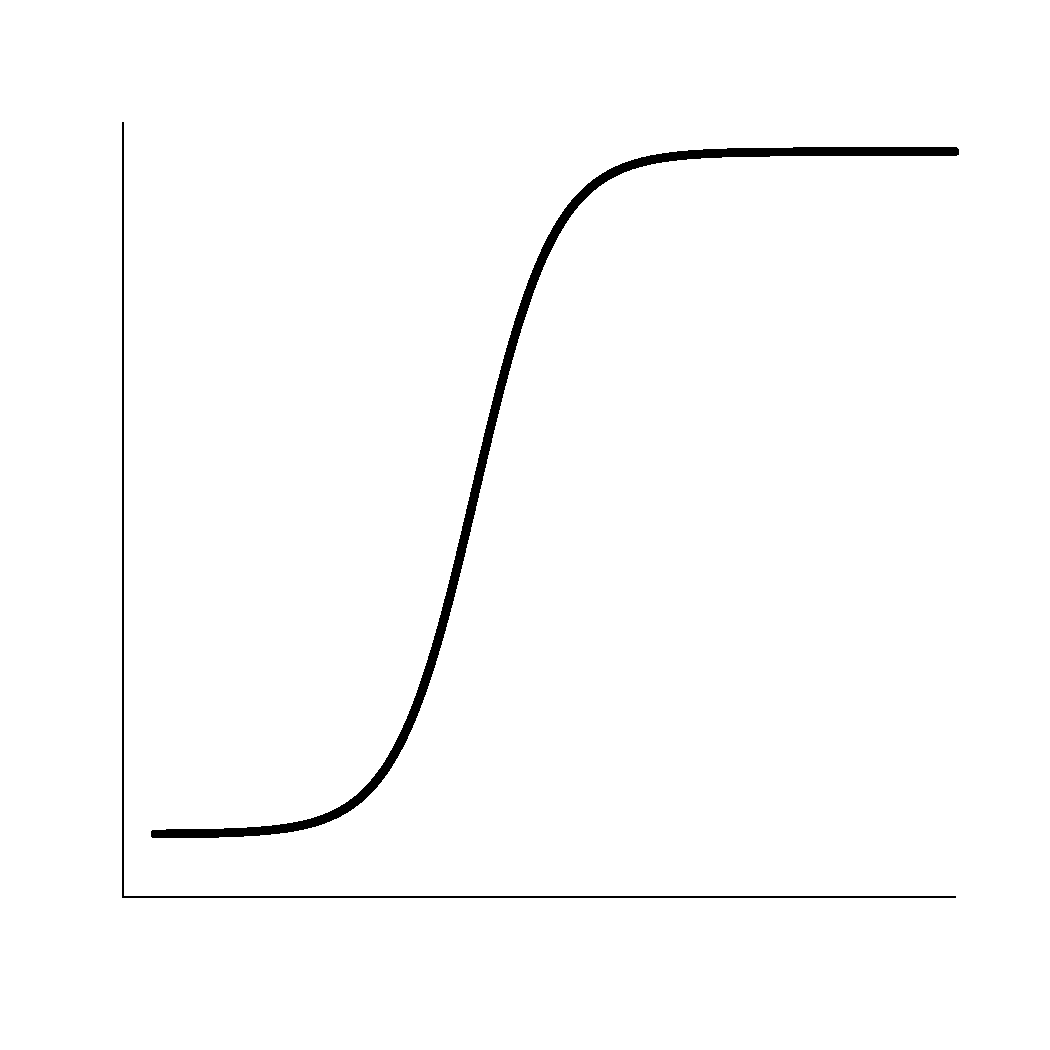
\includegraphics[width=0.45\textwidth]{logistic_a.pdf}} 
    \subfigure[]{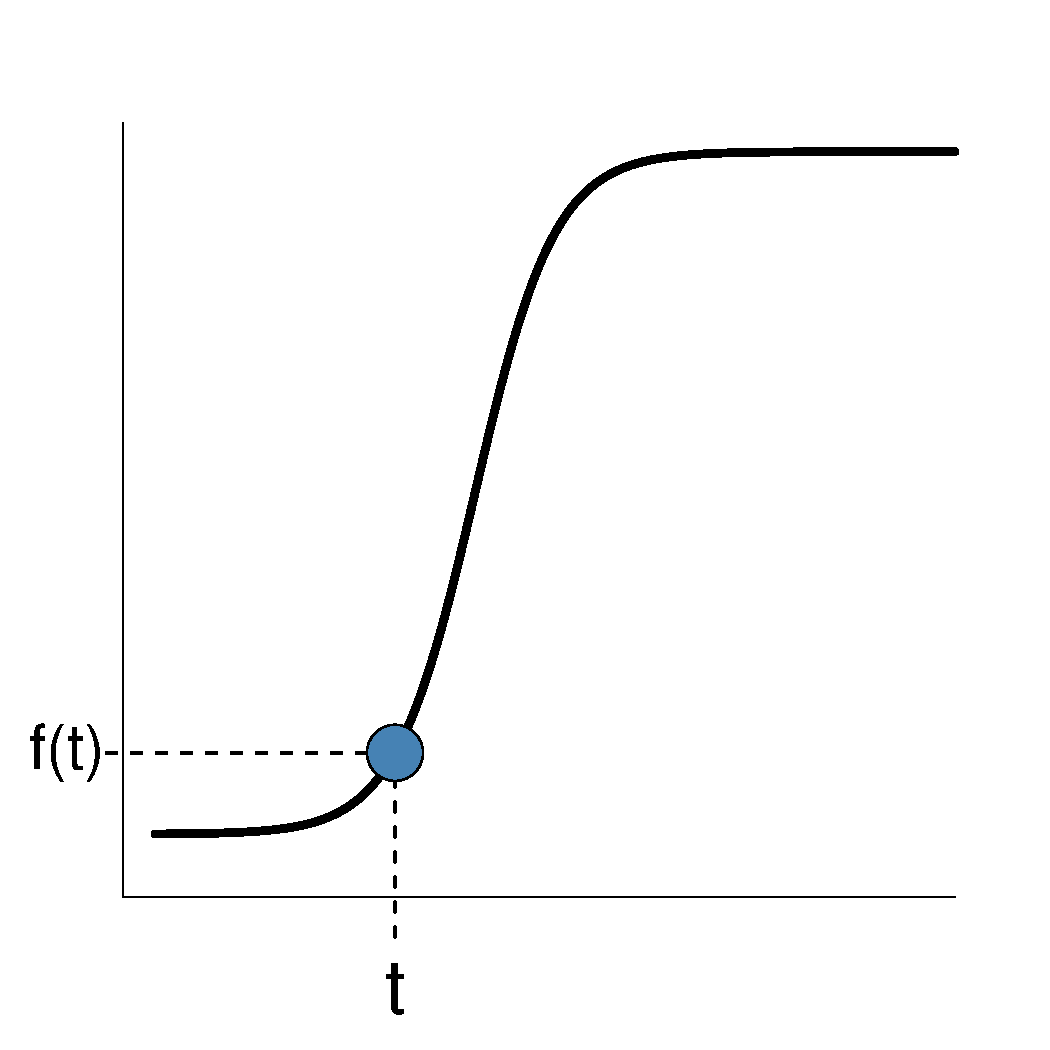
\includegraphics[width=0.45\textwidth]{logistic_b.pdf}} 
    \subfigure[]{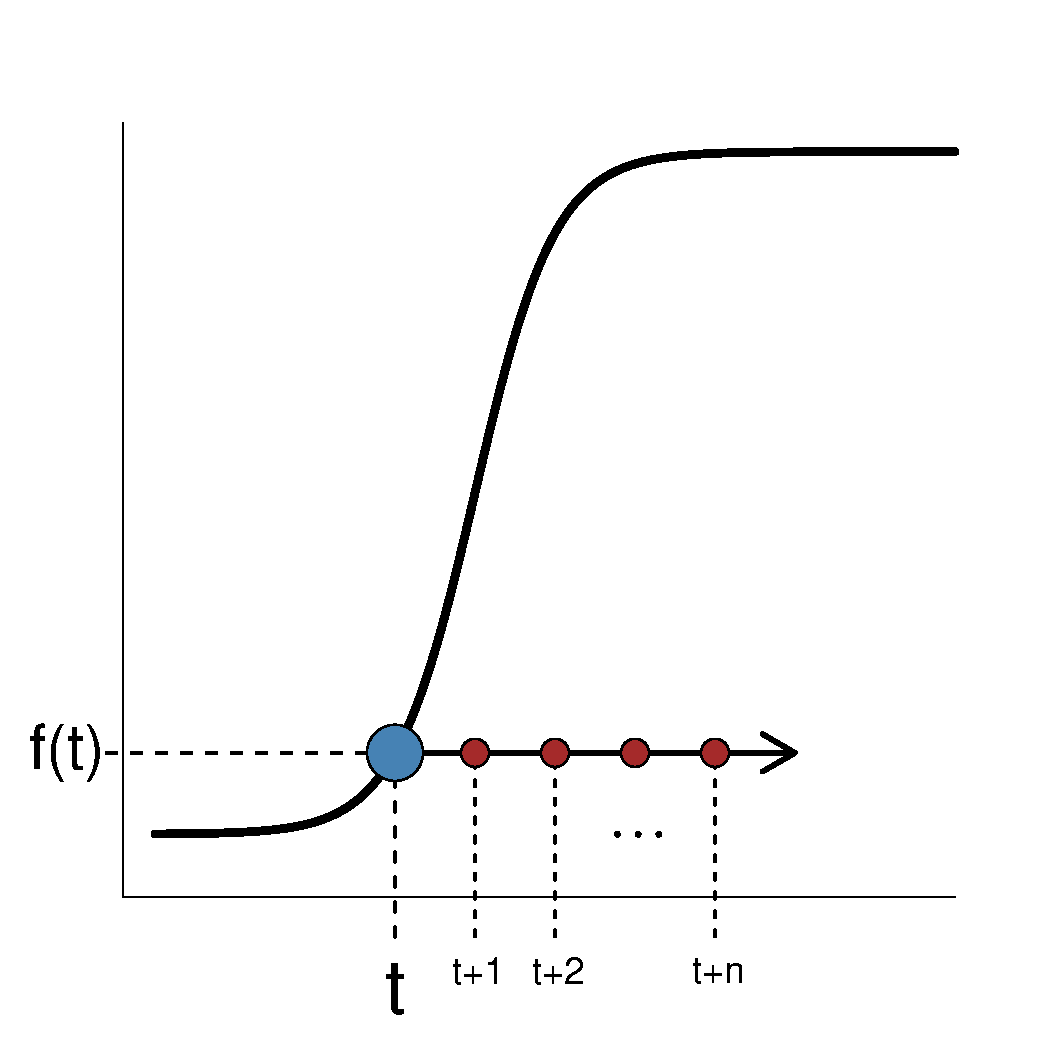
\includegraphics[width=0.45\textwidth]{logistic_c.pdf}}
    \caption{ \textbf{(a.)} Example of a nonlinear activation curve $f(t|\theta)$ \textbf{(b.)} At some time, $t$, a saccade is launched with its destination probabilistically determined by $f(t|\theta)$ \textbf{(c.)} For a look persisting over $n$ time points, $t+1, \dots, t+n$, we are recording ``observed" data, adding to the proportion of fixations at each time but without having gathered any additional observed data at $f(t+1 | \theta), \dots,f(t+n | \theta)$, providing a biased estimate the true probability. }
\label{fig:folly_of_fixation}
\end{figure}

It would be constructive to comment briefly on how the added observation bias would manifest when modeling looks to the Target object, as this is something we will see in a number of simulations following this. As the logistic function modeling the Target is monotonic, it holds that $f(t+1|\theta) > f(t | \theta)$ for all $t$. From the depiction given in Figure~\ref{fig:folly_of_fixation}, we should anticipate that each of the added observations acts to deflate the true probability. Accordingly, we expect two see two distinct phenomenon: first, on account of the true probability being deflated at each time, we should expect the estimate of the slope to be negatively biased (i.e., a flatter slope), and second, we should expect the crossover parameter to be positively biased, on account of the flatter slope and consequent later inflection point. This deflation of values on the $y$-axis should result in what appears to be a horizontal shift along the $x$-axis, and indeed, this is what we will find in each of the cases that follow.

As a final comment here and to reiterate a point previously made, our intent here is not to say that the length of a fixation is irrelevant in consideration of the strength of underlying activation. Rather, we argue that by clearly delineating separate processes we can more concisely recover those that we are interested in.  



\subsection{Delayed Observation Bias}


The final portion of the look onset model is that associated with oculomotor delay. Unlike the situation with the added observation bias, oculomotor delay affects both methods in that the delay between the mechanism of interest and the observed outcome is the same. Previously, we noted that this delay is typically acknowledged to be ``roughly" 200ms, and in a standard VWP analysis it is usually accounted for with a horizontal shift of 200ms to the observed data. The ability to correctly specify and correct for this delay is critical, particularly in situations such as the look onset method in which the total data is much sparser and potentially much more sensitive to misspecification. 

We facilitate this by specifically accounting for the phenomenon of oculomotor delay as a random process, denoted with the variable $\rho$. Under this specification, observe that a look initiated at time $t$ is towards the target not with probability $f(t|\theta)$ but rather $f(t - \rho | \theta)$. The difference between these is what we call the \textit{delayed observation bias}. There are two  qualities of delayed observation bias that we consider here. The first is the simple observation that if there is any difference between the true mean duration of oculomotor delay and 200ms, then the typical adjustment made to correct for it will itself be biased. Assuming that the mean oculomotor delay is 200ms (and there is no observed bias), our second consideration relates to the degree of randomness present and how this variability impacts the recovery of the underlying activation function.

While we don't here provide any specific solutions to this problem (though see future directions in the discussion, as well as the discussion on total variation in the appendix), it will be important to identify the potential impact of this phenomenon and demonstrate the need for further investigation.





\section{Recovery of Individual Curves}\label{sec:ind_curves}



In this section we construct a number of simulations to investigate the impact of added observation bias in the recovery of the underlying activation, as well as highlight the influence of randomness in the oculomotor delay in recovery. The simulations are constructed to emulate a typical study in the Visual World Paradigm, in which individual subjects are tasked with undergoing a series of trials, during each of which subjects make a series of fixations whose locations are probabilistically associated with lexical activation. For brevity, we consider in this section only those fixations associated with the Target object, modeled with the four parameter logistic as given in Equation~\ref{eq:logistic1}; simulations according to looks to competitors is treated in the index, though the phenomenon we detail here are ultimately agnostic to any particular generating function. We will begin by detailing the process of simulating a single subject. 


\begin{figure}[H]
\centering
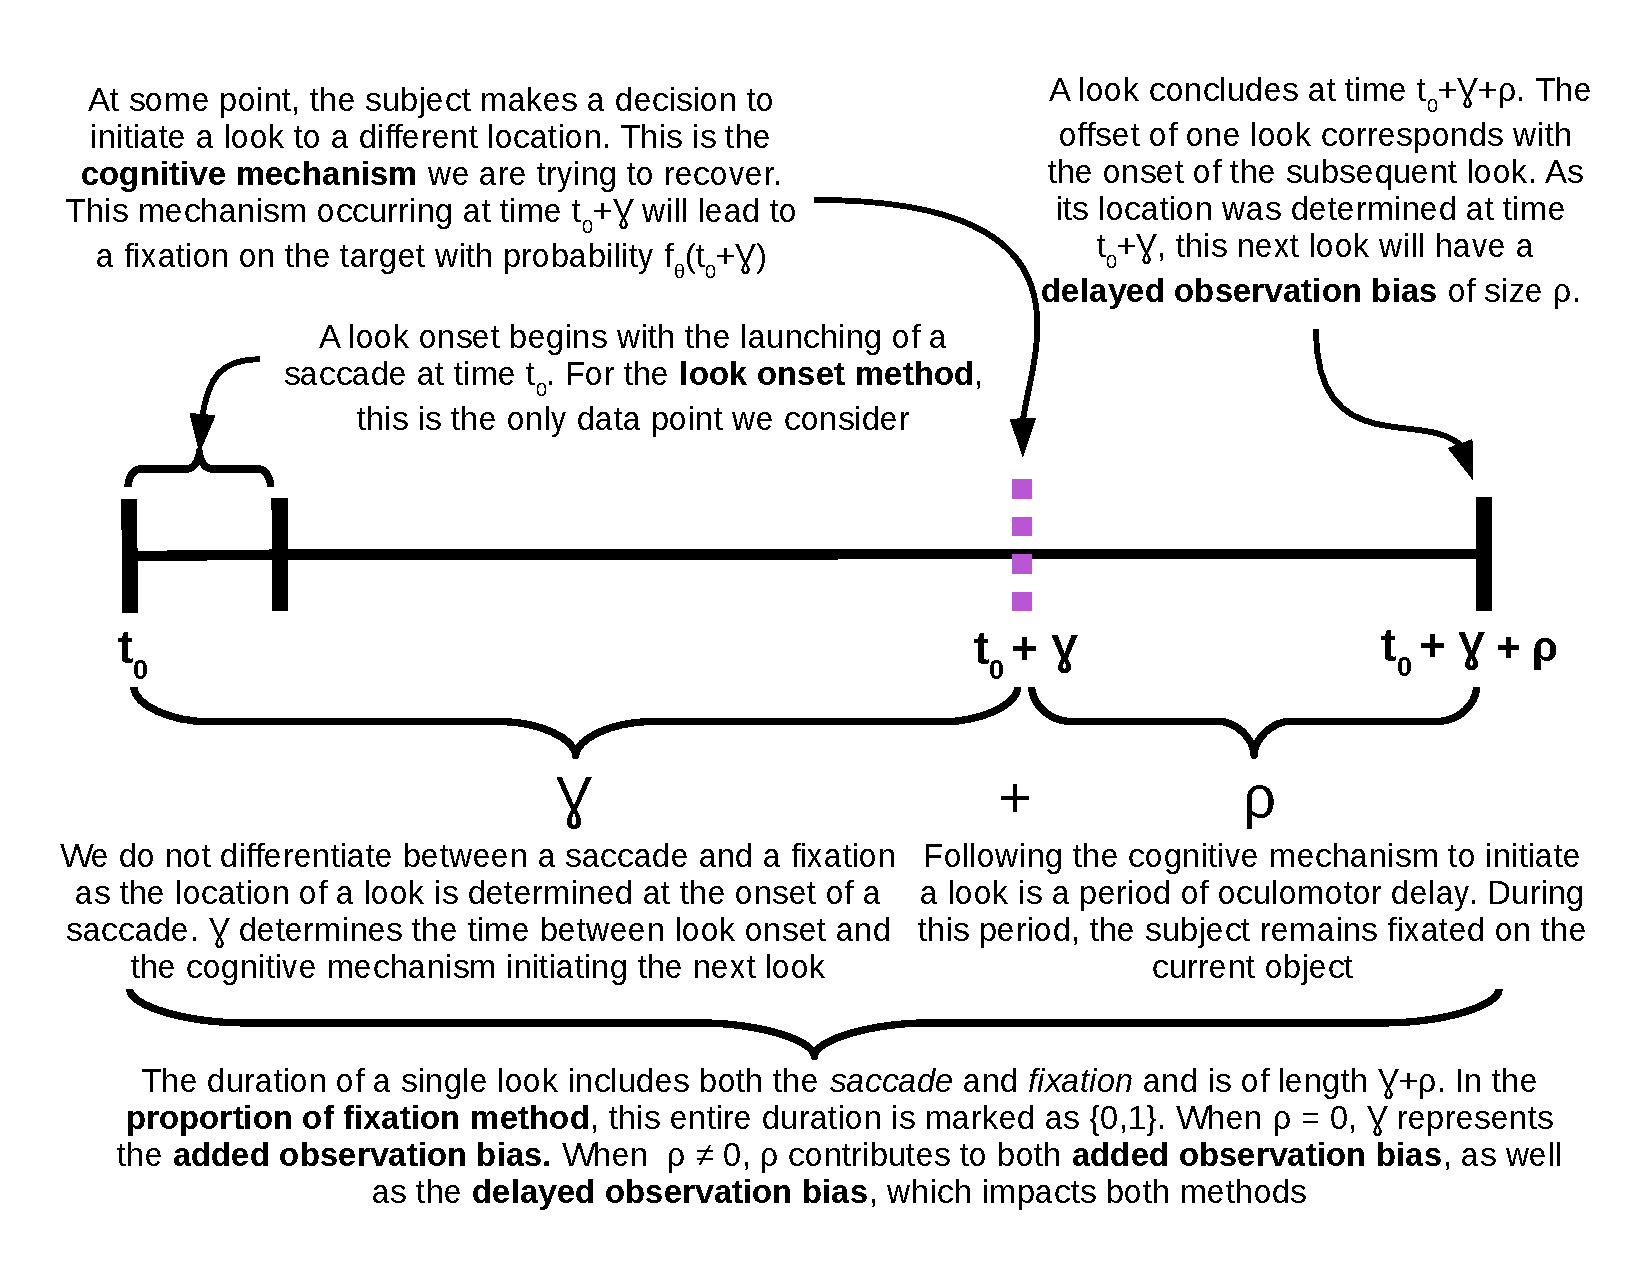
\includegraphics[width=\textwidth]{anatomy_of_look.pdf}
\caption{The Look Onset model}
\label{fig:anatomy_of_look}
\end{figure}


First, each subject $i$ randomly draws a set of parameters $\theta_i$ from an empirically determined distribution based on normal hearing participants in the VWP \citep{FarrisTrimble2014} to construct a subject specific generating curve, $f(\cdot | \theta_i)$, where $f$ here is assumed to be the logistic given in Equation~\ref{eq:logistic1}.  It is according to this function that the decision to initiate a look at time $t$ will subsequently direct itself to the Target with probability $f(t|\theta_i)$. We then go about simulating trials according to the following method: At some time $t_0$, a subject initiates a look. This look persists for at least a duration of $\gamma$, drawn from a gamma distribution with mean and standard deviation independent of time and previous fixations. At time $t_0+\gamma$, the subject determines the location of its next look, with the next look being directed towards the target with probability $f(t+\gamma | \theta_i)$. The decision to initiate a look is followed by a period of oculomotor delay, $\rho$, during which time the subject remains fixated in the current location. Finally, at time $t_0 + \gamma + \rho$, the subject ends the look initiated at $t_0$ and immediately begins its next look to the location determined at time $t_0 + \gamma$. For the look onset method, the only data recorded are the times of a look onset and their location: in this case, at times $t_0$ and $t_0 + \gamma + \rho$. By contrast, the proportion of fixation method records the object of fixation at 4ms intervals for the entire period of length $\gamma + \rho$. A single trial begins at $t = 0$ and continues constructing looks as described until the total duration of looks exceeds 2000ms. Each subject undergoes 300 trials, and 1,000 subjects are included in each simulation.

Three total simulations were performed to investigate the biases identified in the previous section, each differing only in the random distribution of the oculomotor delay parameter, $\rho$. In the first simulation we set $\rho = 0$ to remove any oculomotor delay. Under this scenario, a look initiated at time $t$ by subject $i$ will be directed towards the target with probability $f(t|\theta_i)$. Doing so removes any potential bias from delayed observation and allows us to identify the effects of the added observation bias in isolation. In the remaining simulations we probe the effects of randomness in oculomotor delay, investigating what effect uncertainty may have in our recovery of the generating function. We do this assigning $\rho$ to follow either a normal or Weibull distribution, each with a mean value of 200ms. As is standard in a VWP analysis, we subtracted 200ms from each observed point prior to fitting the data. A consequence of this is that in these simulations, the bias itself is accurately accounted for by subtracting the correct mean, with the resulting error in the curve fitting process the result of the inherent variability. This does not detract from the argument being made, however, and any true bias in the mean of the oculomotor delay would asymptotically result in a horizontal shift of the observed data according to the direction and magnitude of the bias.

Simulated data was fit to the four parameter logistic function using \xt{bdots v2.0.0}.

As all of the data could not be individually inspected prior to being included in the analysis, subjects were excluded from consideration if fitted parameters from either the look onset method or the proportion of fixation method resulted in a peak less than the slope, or if the crossover or slope were negative. In the settings in which there was no delay, normally distributed delay, or Weibull distributed delay, 981, 973, and 981 subjects were retained, respectively.


\subsection{Results}

Presented together are results from each of the simulations, beginning first with a collection of visual summaries. Simulation settings under each of the assumptions for oculomotor delay are displayed as a panel in Figure~\ref{fig:panel_no_delay},~\ref{fig:panel_normal_delay}, and~\ref{fig:panel_weibull_delay}. Each panel starts with a box plot showing the observed bias $(E(T) - \theta)$ for each of the retained subjects. Following this is a representative sample of subject-specific curves under each method, alongside error curves demonstrating the difference between the generating and recovered curves. 

The results presented for no oculomotor delay in Figure~\ref{fig:panel_no_delay} serve to highlight the impact of the added observation bias in isolation, and from this we observe a few things. As predicted, we see positive bias in the crossover parameter for the look onset method, consistent with the observation that the majority of ``observations" are underestimates of the true probability (as would be true in all monotone functions). As more time passes before the inflection point is reached, this has the secondary effect of ``flattening" the estimated curve, an effect that we also see with the slight negative bias present in the slope parameter. In contrast, the recovery of each of the parameters under the look onset method appear to be unbiased.

These observations are again reflected in the presentation of representative curves, in all cases resulting in a curve estimated from the proportion of fixation method that is horizontally shifted right of the generating curve and also less steep. There is an interesting phenomenon whereby the horizontal shift in the representative curves visually appears to be a small difference -- however, the bias between the true and recovered curves is not horizontal but vertical, and the magnitude of error between these is more obviously demonstrated in the representative error curves making up the last portion of the panel. This is especially important considering the fact that it is precisely this portion of the curve that is most sensitive to bias in recovery. The consequences of this are discussed briefly in the appendix. 

For the remaining panels, we see that the primary effects of oculomotor delay are that of increased variability in the recovery of parameters. We also see evidence of bias in the recovery of all parameters for \textit{both} methods in the case of Weibull delay, demonstrating that even when we make unbiased adjustments for oculomotor delay as we did here, the highly non-linear nature of these curves can result in downstream difficulties. This especially highlights the need for effectively addressing the effects of variability in oculomotor delay.

\begin{figure}[H]
\centering
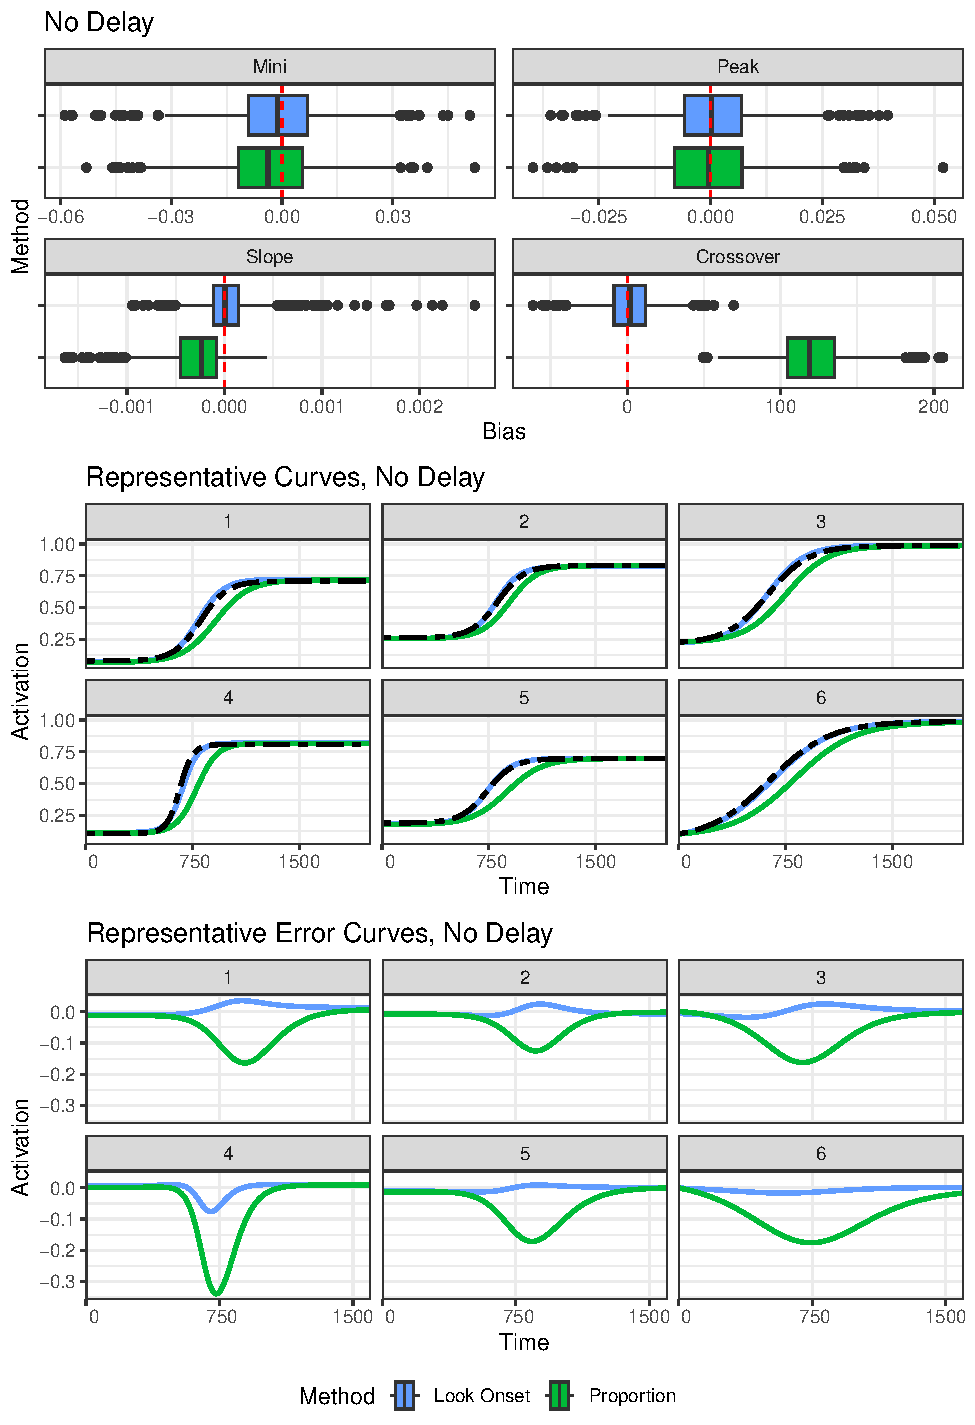
\includegraphics{rep_and_diff_no_delay.pdf}
\caption{Summary of simulation results in the recovery of subject-specific curves generated by the logistic function with no oculomotor delay}
\label{fig:panel_no_delay}
\end{figure}


\begin{figure}[H]
\centering
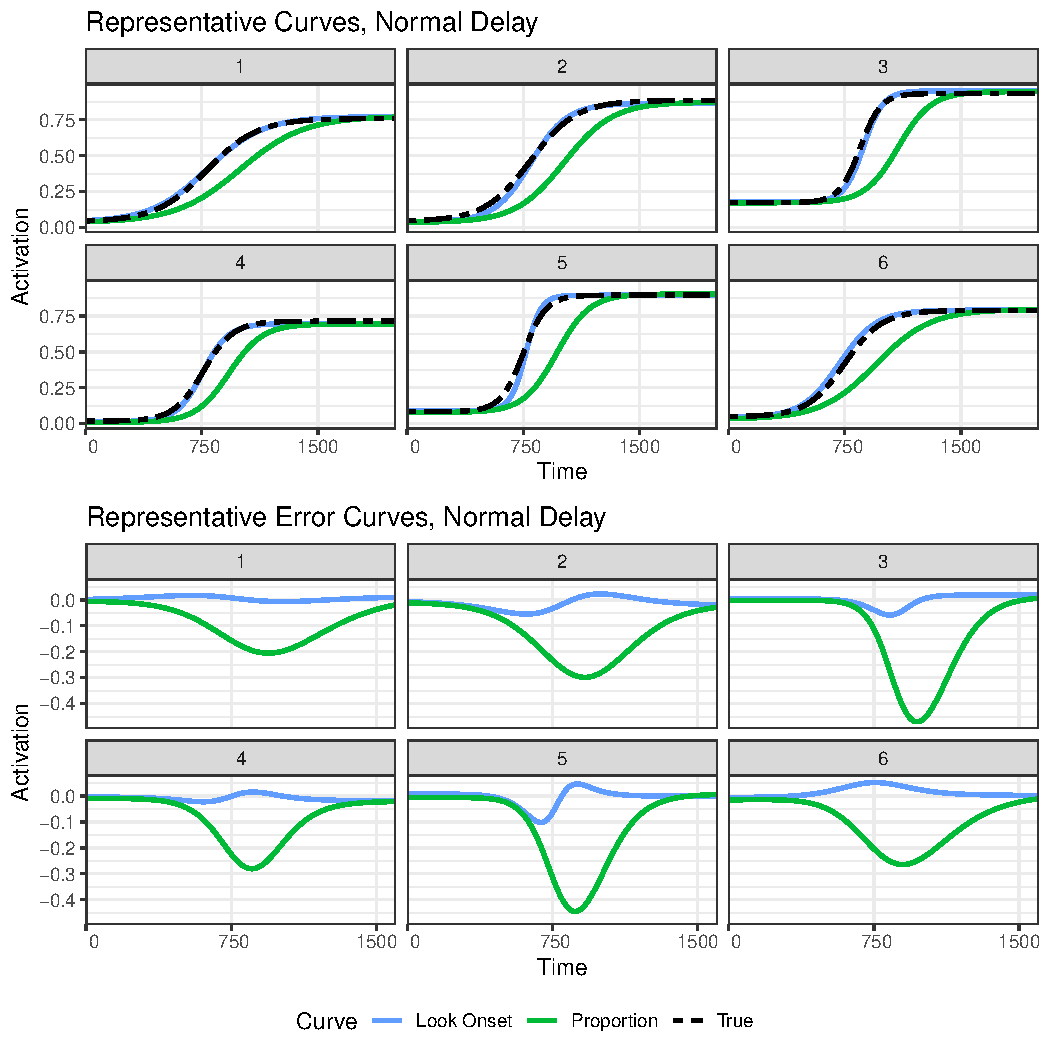
\includegraphics{rep_and_diff_normal_delay.pdf}
\caption{Summary of simulation results in the recovery of subject-specific curves generated by the logistic function with normally distributed oculomotor delay}
\label{fig:panel_normal_delay}
\end{figure}



\begin{figure}[H]
\centering
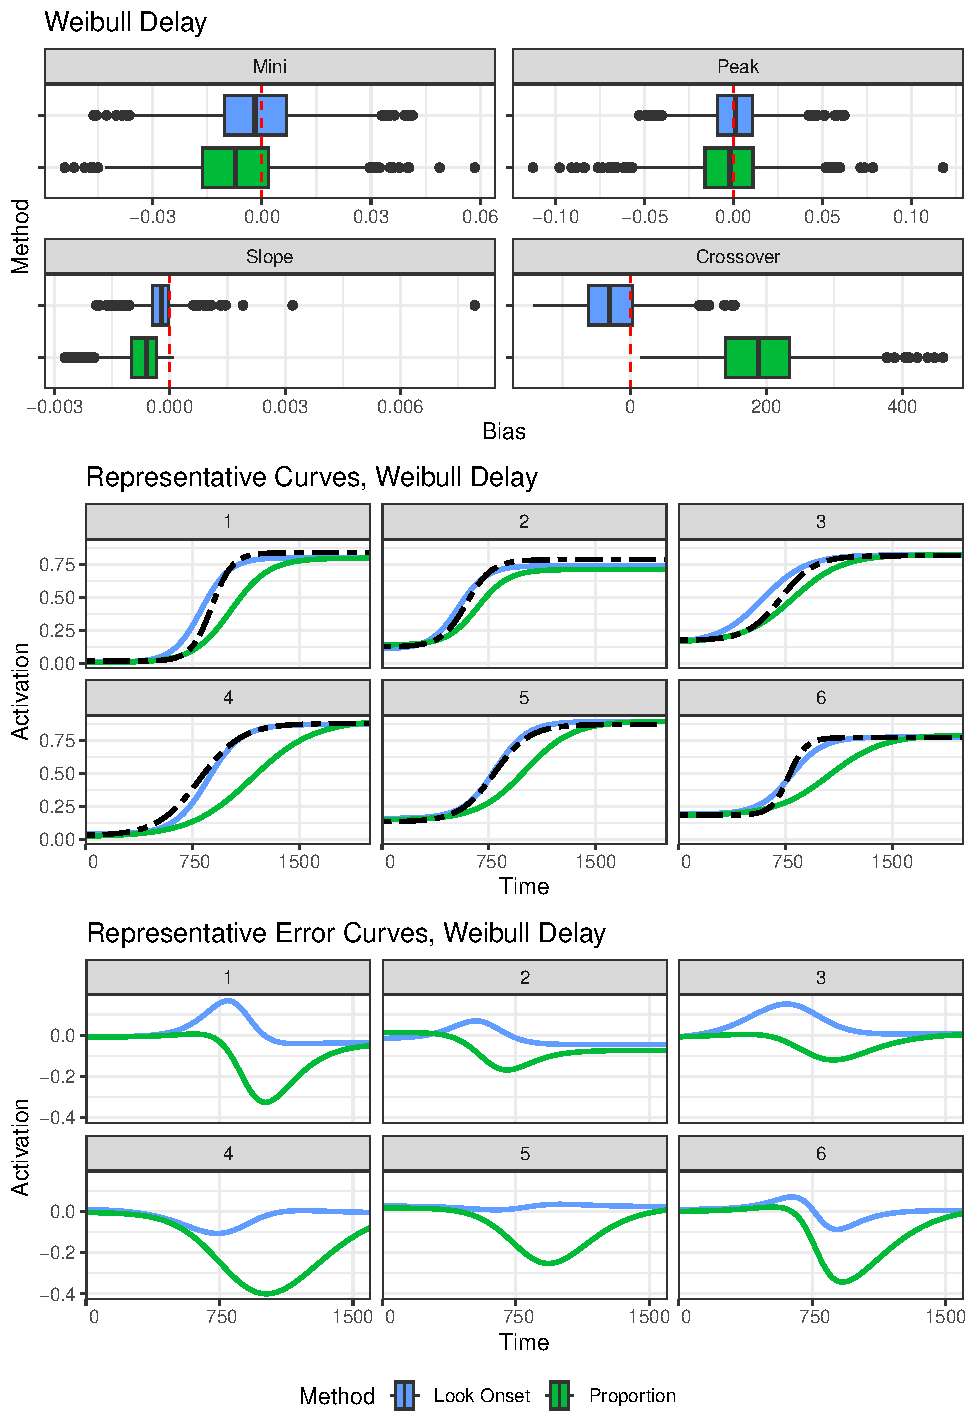
\includegraphics{rep_and_diff_weibull_delay.pdf}
\caption{Summary of simulation results in the recovery of subject-specific curves generated by the logistic function with Weibull distributed oculomotor delay}
\label{fig:panel_weibull_delay}
\end{figure}



In addition to the visual summaries, we present in Table~\ref{tab:mise_sims} a summary of the mean integrated squared error (MISE) between the generating and recovered curves using each of the methods

We begin by noting the  magnitude of difference between the look onset method and the proportion of fixation method in the case of $\rho = 0$, or No Delay, demonstrating the amount of bias introduced in the proportion method. This alone demonstrates how critical of an issue the added observation bias is in the recovery of the underlying activation.

To assess the effects of randomness in the oculomotor delay, it seems prudent to limit the comparisons within each method. Considering first the look onset method, we see that as the degree of variability increases, so does the difficulty in correctly recovering the underlying curve. It is important to note that these magnitudes are meant to be relative rather than absolute: the particular values observed are a function of the relationship between the generating $\gamma$ distribution and that of $\rho$. Nonetheless, this does suggest a need to further investigate ways to control for the added uncertainty. To quickly comment on the apparently ``flipped" MISE for the proportion of fixation method as it relates to the normal and Weibull distributed oculomotor delay, it would seem as if the skew of the Weibull distribution acted in such a way as to actually offset some of the observed added observation bias and seems more an artifact of the simulation conditions rather than an inherent statement relating OM bias to the proportion of fixation method in general.

% latex table generated in R 4.2.2 by xtable 1.8-4 package
% Wed Feb  8 15:10:31 2023
\begin{table}[H]
\centering
\begin{tabular}{llrrr}
  \hline
Method & Delay & 1st Qu. & Median & 3rd Qu. \\ 
  \hline
Look Onset & No Delay & 0.17 & 0.32 & 0.56 \\ 
  Look Onset & Normal Delay & 0.37 & 0.71 & 1.24 \\ 
  Look Onset & Weibull Delay & 1.05 & 2.16 & 4.23 \\ 
  Proportion & No Delay & 8.21 & 11.33 & 16.01 \\ 
  Proportion & Normal Delay & 22.90 & 30.65 & 39.37 \\ 
  Proportion & Weibull Delay & 15.27 & 24.75 & 38.14 \\ 
   \hline
\end{tabular}
\caption{Summary of mean integrated squared error across simulations}
\label{tab:mise_sims}
\end{table}

Overall, these results conclusively demonstrate both the devastating effect of added observation under the assumptions illustrated in Figure~\ref{fig:anatomy_of_look} as well as the need to consider the effects of variability associated with oculomotor delay, even when unbiased adjustments are able to be made. 


\section{Recovery of Group Differences}



In Section~\ref{sec:ind_curves}, we demonstrated the utility of the look onset method in the asymptotic recovery of individual curves under our generative model. Often, however, the need to specify subject-specific differences is in pursuit of a higher goal, namely the identification of clinically relevant differences between groups. This problem is elaborated upon in \citet{mcmurray2010individual}, where it is noted, for example, that simply averaging across participants data has the ability to either create or mask group-level effects (i.e., large variability in the crossover parameter in the logistic function in Equation~\ref{eq:logistic1} could manifest in the aggregate as a difference in slope). Having demonstrated the efficacy in recovering the subject-specific curves, we now consider if differences at the subject level are preserved in the aggregate through a power analysis using each of the methods discussed for identifying clinically relevant group differences. 

\begin{figure}[H]
    \centering
    \subfigure[]{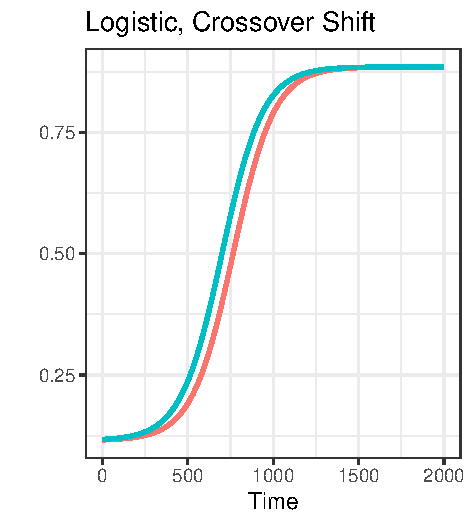
\includegraphics[]{logistic_shift.pdf}} 
    \subfigure[]{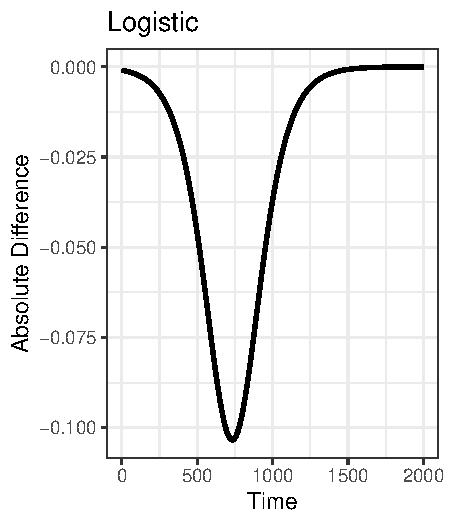
\includegraphics[]{logistic_difference.pdf}} 
    \caption{Plot of logistic groups with horizontal shift, alongside difference curve}
\label{fig:logistic_shift}
\end{figure}



We proceed just as we did in Section~\ref{sec:ind_curves}, generating data according to the process previously described and detailed in Figure~\ref{fig:anatomy_of_look}, recovering individual curves via each the look onset and proportion of fixation methods. What differs here, however, is that each simulation is constructed to simulate drawing two groups with 25 subjects each from empirically estimated distributions that differ from one another as a horizontal shift of 65 in the location parameters (i.e., the crossover parameter in the logistic and the mean parameter in the asymmetric Gaussian). An illustration of the mean structure of each group and its shifted counterpart is depicted in Figures~\ref{fig:logistic_shift} and~\ref{fig:dg_shift} for the logistic and asymmetric Gaussian, respectively.

\begin{figure}[H]
    \centering
    \subfigure[]{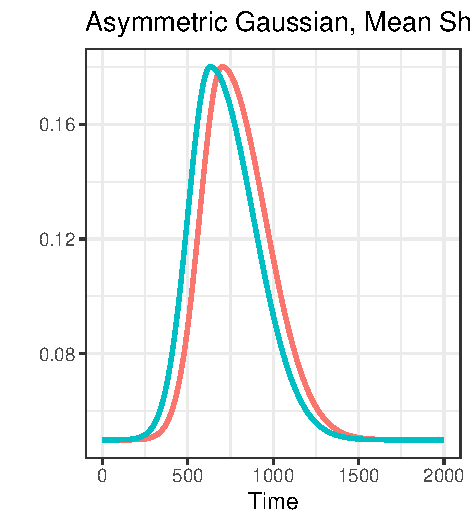
\includegraphics[]{dg_shift.pdf}} 
    \subfigure[]{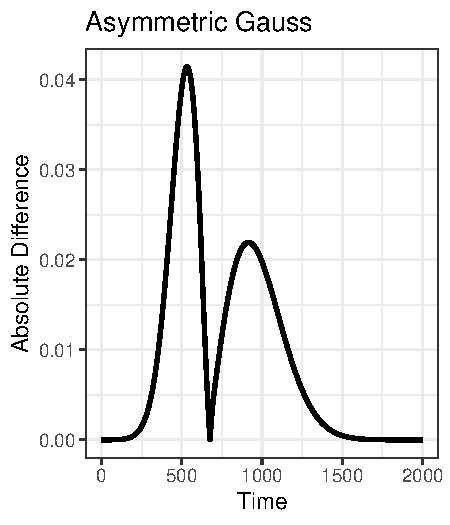
\includegraphics[]{dg_difference.pdf}} 
    \caption{Plot of asymmetric Gaussian groups with horizontal shift, alongside difference curve}
\label{fig:dg_shift}
\end{figure}

Just as in the case of the recovery of subject-specific curves, what we are interested in here is the identification of vertical differences between groups, the magnitude of which at each time point is given in Figures~\ref{fig:logistic_shift} and~\ref{fig:dg_shift} as well. As greater differences should be easier to detect, we should anticipate a strong temporal relationship between the magnitudes of difference  and the observed power.

Power for these methods is estimated in the following way: first, we simulate two groups of 25 subjects each by drawing function parameters from either the empirically determined multivariate normal distribution used in Section~\ref{sec:ind_curves} or from that same distribution with the location parameter shifted horizontally by 65. We proceed exactly the same way, both in recovering the curves under the look onset and proportion of fixation method, and under conditions with no oculomotor delay, as well as Normally distributed and Weibull distributed delay. The fitted subject-specific curves are then used to create an estimate of the group distribution using the bootstrapping procedure in the \xt{bdots} package. Using the \xt{p\_adjust = "oleson"} adjustment for the nominal alpha, temporal regions identified as statistically significant are recorded. We repeat this process 1000 times, taking at each 4ms time point the proportion of instances in which statistically significant differences were identified.



\subsection{Results}

\begin{figure}[H]
\centering
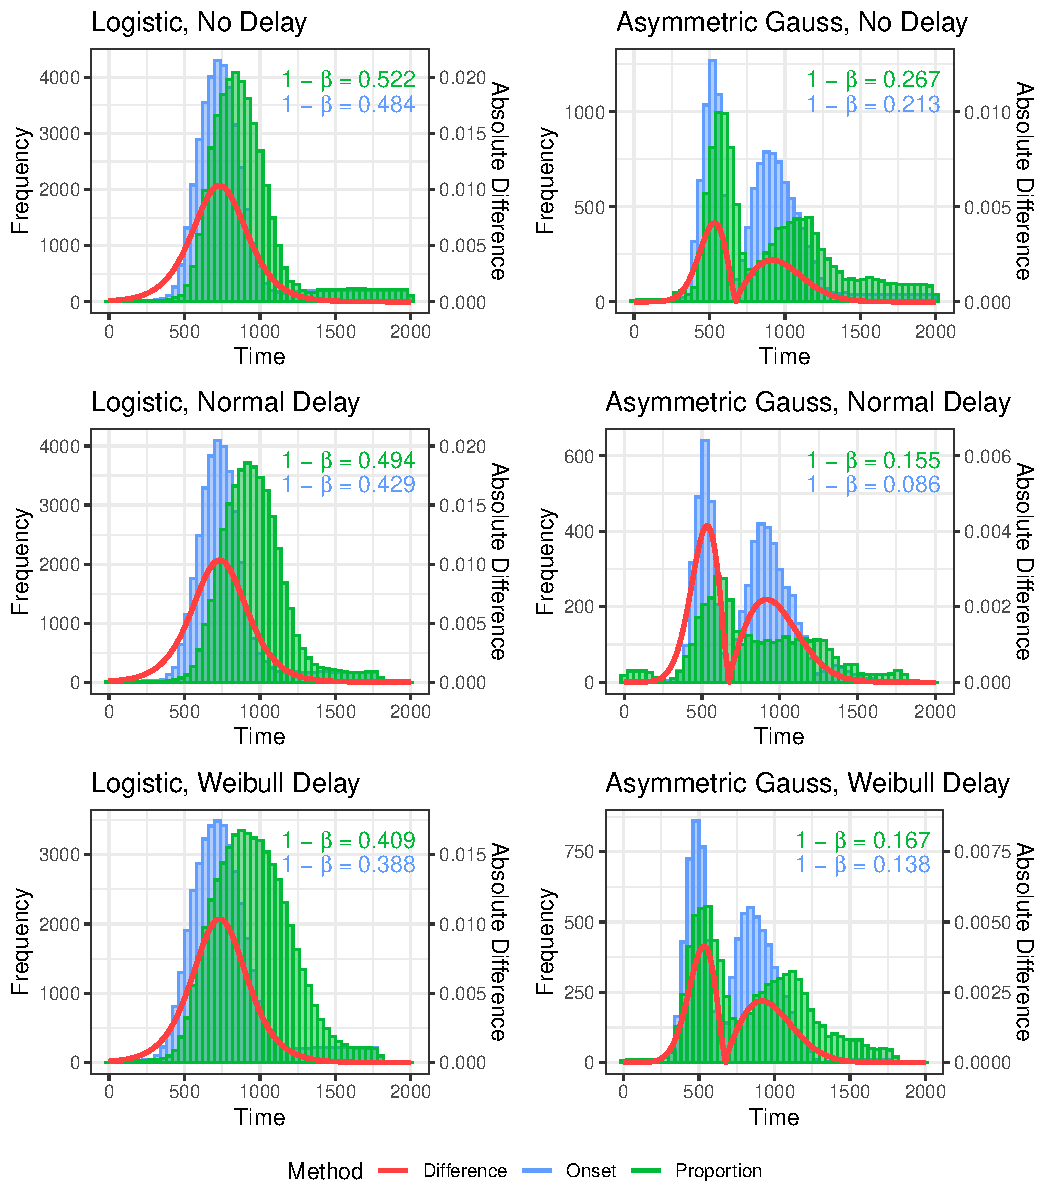
\includegraphics{diff_hist_all.pdf}
\caption{Histograms of observed power and overlaid error function}
\label{fig:diff_hist_all}
\end{figure}


Results of the simulations are presented visually in Figure~\ref{fig:diff_hist_all}. Within each tile is a histogram indicating the proportion of trials in which a statistically significant difference was identified\footnote{Binwidth for each histogram is 40, which is why some proportions are greater than 1000}. Laid over each histogram are plots of the error curves from Figures~\ref{fig:logistic_shift} and~\ref{fig:dg_shift}, helping to coordinate observed power in time. In the top right of each histogram is an estimate of total power, indicating the proportion of simulations in which \textit{any} difference was identified. Finally, the correlation between the error curve and power density for each of the setting simulations is provided in Table~\ref{tab:correlation_power}.


\begin{table}[H]
\centering
\begin{tabular}{llcc}
  \hline
Curve & Delay & Look Onset & Proportion of Fixations \\ 
  \hline
Logistic & No Delay & 0.9527 & 0.7789 \\ 
  Logistic & Normal Delay & 0.9503 & 0.5390 \\ 
  Logistic & Weibull Delay & 0.9861 & 0.6404 \\ 
  Asymmetric Gauss & No Delay & 0.9520 & 0.6554 \\ 
  Asymmetric Gauss & Normal Delay & 0.9359 & 0.6448 \\ 
  Asymmetric Gauss & Weibull Delay & 0.9413 & 0.8681 \\ 
   \hline
\end{tabular}
\caption{Correlation of power density with difference function between methods}
\label{tab:correlation_power}
\end{table}

There are several conclusions that can be readily drawn from the results presented. First, Figure~\ref{fig:diff_hist_all} demonstrates that in each case, the observed overall power was greater for the look onset method. In conjunction with this is the observation that the magnitude of temporal power in the look onset method closely matches the magnitude of absolute difference, which is corroborated by the correlations presented in Table~\ref{tab:correlation_power}. A corollary of this observation is that clinically relevance differences that are detected by the proportion of fixation method may be temporally misaligned. 




\section{Application to Real Data}

While improved performance in the theoretical domain is a necessary condition for the adoption of the look onset method, it is not sufficient, and towards that end we turn our attention now to an application with real data. We revisit here a study conducted by \cite{mcmurray2010individual}, which collected VWP data on 93 children differing in language and cognitive abilities. This included children who were typically developed (N, $n = 40$), those with specific language impairment (SLI, $n = 20$) and non-specific language impairment (NLI, $n = 17$), and those with specific cognitive impairment (SCI, $n = 16$). Though the primary goals of this study involved both the investigation of individual differences and the mapping of particular physiological characteristics to TRACE parameters, we limit our consideration here to a standard analysis in \xt{bdots} whereby we seek to identify temporal-specific differences in the trajectory of fixations with looks to the Target, modeled with the four parameter logistic function. We do this by structuring the original data according to both the proportion of fixations and look onset methods, fitting subject-specific curves to the data, and then identifying statistically significant differences via permutation testing in \xt{bdots}. As there are four total groups, we consider each of the pairwise differences, resulting in six total differences for investigation.

\subsection{Data Preparation}

There are a number of decisions that must be made when transforming raw eye tracking data to a format suitable for the look onset method. Briefly, we detail here the decisions made in processing data for both the proportion of fixations and for look onset. First, in all cases we removed trial data in any trials for which the subject made no fixations or selected the incorrect object in response to the auditory signal. We recorded no fixations or saccade movements (for look onset) that occurred past 2300ms, and we truncated data in each trial to end once the participant had selected the correct response.

For look onset data specifically, there are a number of additional decisions to be made, particularly regarding the beginning and end of an individual trial. At the beginning of a trial when $t = 0$, for example, the eyes are already fixated on some location (typically the center), yet these are accounted for in the proportion of fixation. Regarding look onset, we must then decide whether we choose to take the first saccade launched after the beginning of the trial, resulting in a paucity of data near the beginning, or to choose to include the first saccade launched prior to the beginning of the trial which would be unrelated to the auditory stimulus (as it had not yet been received), but would offer more consistency with the data provided via the proportion of fixations. Similarly, one notes that at the end of a trial, a fixation will persist until the response has been collected (resulting in ``observed" data), whereas the final saccade launched prior to response will often be a few hundred milliseconds sooner, resulting in a similar paucity of data at the end of the trial. Ultimately, we elected to only include saccades launched after the onset of auditory stimulus and made no further accommodation for the end of the trial, and although our results were not sensitive to either of these decisions, we believe they are worth consideration in future work.


\subsection{Results}

\begin{figure}[H]
    \centering
    \subfigure[]{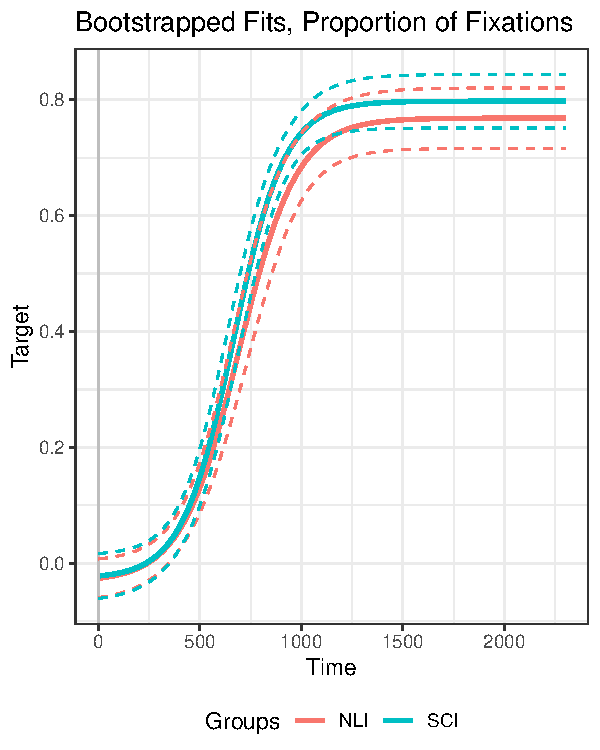
\includegraphics[width=0.48\textwidth]{irl_data_prop_1.pdf}}
    \subfigure[]{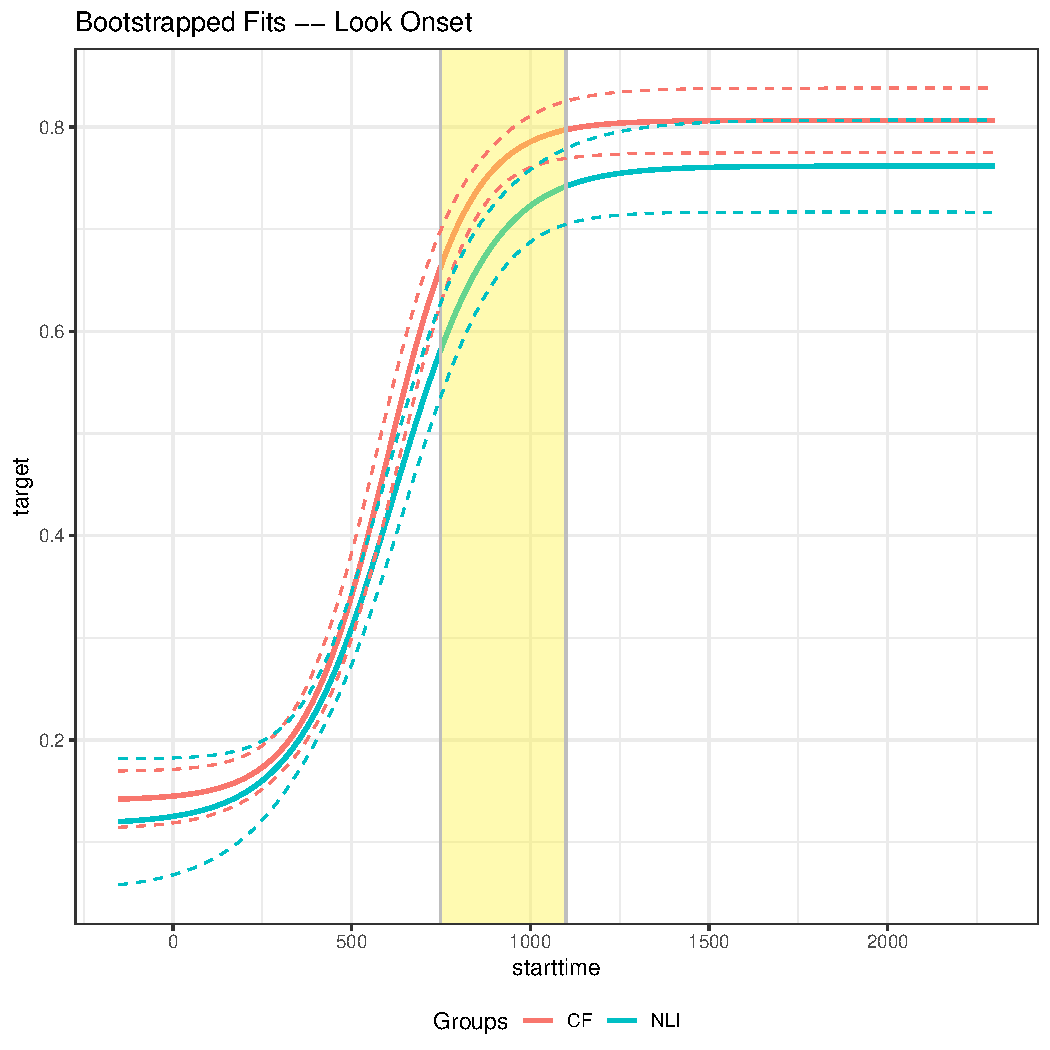
\includegraphics[width=0.48\textwidth]{irl_data_onset_1.pdf}}
    \caption{Estimated mean curves with confidence intervals of NLI and SCI, with significant region identified using the look onset method}
\label{fig:irldata1}
\end{figure}

Temporal differences between groups were made using permutation testing in \xt{bdots}. Of the six comparisons made, only two were found to have significant differences between group curves, those being the comparisons made between specific cognitive impairment (SCI) and non-specific language impairment (NLI), as well as between NLI and typically developed adolescents (N). Further, these differences were only identified with the look onset method, with the proportion of fixation method in both cases offering null results. Plots of the mean curves and bootstrapped confidence intervals, along with highlighted regions of identified differences, are provided in Figure~\ref{fig:irldata1} and Figure~\ref{fig:irldata2}.



\begin{figure}[H]
    \centering
    \subfigure[]{
\includegraphics[width=0.48\textwidth]{irl_data_prop_2.pdf}}
    \subfigure[]{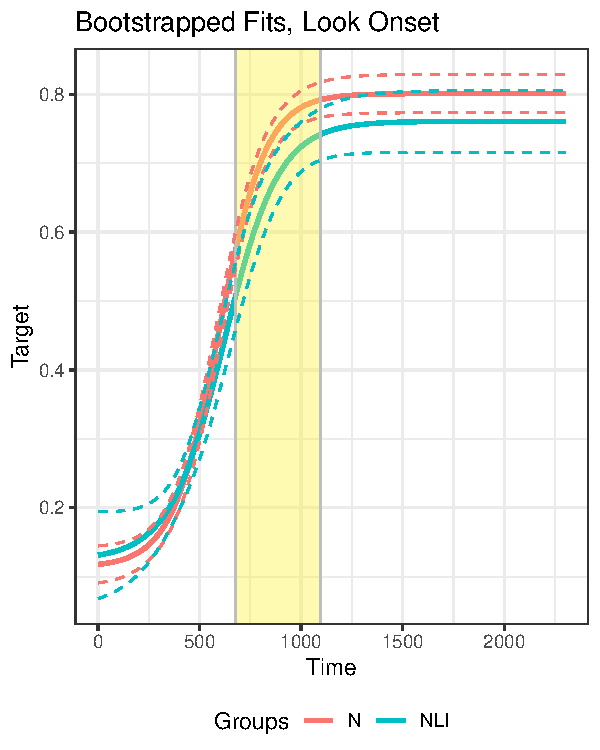
\includegraphics[width=0.48\textwidth]{irl_data_onset_2.pdf}}
    \caption{Estimated mean curves with confidence intervals of NLI and N, with significant region identified using the look onset method}
\label{fig:irldata2}
\end{figure}



\section{Discussion}



Through our investigation, we have presented a physiologically grounded model relating eye tracking data to underlying lexical access by placing emphasis singularly on the first instance of a look. Under the assumptions of this model, we further demonstrated a significant source of bias present under the standard ``proportion of fixations" method typical of VWP data. We have proposed an alternative in response, the look onset method, which limits relevant data to the initial launching of a saccade. Under our generative model, we not only demonstrated superior recovery of individual subject-specific curves but also in the unbiased identification of temporal-specific differences between groups. The utility of this additional power was made evident in our re-examination of an existing study, in which the look onset method identified several statistically significant differences between groups, whereas the proportion of fixation method did not. And finally, the look onset method can be implemented immediately, utilizing the same analytic approach provided by the \xt{bdots} package in R.

The look onset method has the further benefit of giving rise to a much sparser dataset, providing a more computationally tractable basis for algorithms with complexity that scale in the number of observations. This may be of considerable advantage in fitting mixed models to the data, potentially providing the ability to control for trial-specific variability, an option that has hitherto been infeasible. 

Of likely concern to many readers will be the fact that, as the look onset method retains only the initial onset of a fixation, a great deal of information is lost concerning the \textit{duration} of the fixation. It is well established \citep{Salthouse1980} that the length of a fixation is itself meaningful, with longer fixations generally associated with stronger activation. The length of fixation may also be important when attempting to differentiate fixations associated with searching patterns (i.e., what images exist on screen?) against those associated with consideration (is this the image I've just heard?). It would be incorrect to suggest that the look onset method considers the length of fixation \textit{irrelevant}; rather, it makes no statement about it at all. In other words, by clearly delineating two separate processes, one initiating an eye movement, the other determining the duration, we free ourselves to construct far more nuanced models. For example, the length of a fixation may suggest a weighting to the proceeding look onset, with a longer duration being indicative of intentional consideration and shorter ones being suggestive of searching behavior. These questions suggest a number of experimental designs to differentiate eye tracking behavior, particularly with regards to scanning/search behavior and experimental conditions, similar to what is demonstrated in \citet{Apfelbaum2021}.


It is also critical to specify a present shortcoming in how the duration of fixations are treated. Implicit in the proportion of fixations method is a crucially overlooked assumption of a linear relationship between the fixation length and the activation. That is, insofar as the construction of the fixation curve is considered, a fixation persisting at 20ms after look onset (and well within the refraction period in which no new information regarding the cognitive mechanism or voluntary fixation could be obtained, see Figure~\ref{fig:whats_in_a_look}) is considered identical to a fixation persisting at 500ms after onset: both are undifferentiated in being recorded as either a $0$ or $1$. In other words, the specific duration of a particular fixation does not directly change how the data is recorded. This is in contrast to the possibility offered by the look onset method, whereby the duration of the fixation could weight the look onset by importance.

A second consideration necessary for using the length of a fixation is the composition of the fixation itself, given in Figure~\ref{fig:whats_in_a_look}. Suppose, for example, that the refractory period following each fixation was exactly 100ms and that the oculomotor delay before initiating the subsequent fixation is exactly 200ms. From this, we could conclude that 300ms of any fixation are ``built in" and have no necessary information regarding the strength of activation motivating the fixation. Without considering this information, we may determine a fixation of 500ms to be 25\% greater than a fixation of 400ms. However, once we account for the ``built in" portion of a fixation, we see that the first is associated with an intentional fixation period of 200ms, whereas the second has an intentional period of only 100ms. In this light, the first fixation might be considered 100\% greater than the latter. And while we offer no more than speculation here, this phenomenon should be taken into consideration in future research.

In conclusion, we have presented a statistically defensible generative model for eye movements in the context of the Visual World Paradigm, accompanied by a novel method for aggregating and analyzing collected data. While the methods proposed are not a drastic alteration to the motivating assumptions of \citet{allopenna1998tracking}, we believe them to be a critical step forward towards a statistically sound treatment of eye tracking data in the realm of lexical activation.




\section*{Appendices}


\section{Misc OM Discussion}


Outside of a demonstration of its existence and potential consequence, little more has been said about addressing the delayed observation bias. Further, the consequences of the delayed observation (under the assumption that the mean value is correctly accounted for) seem almost trivial in comparison to the differences between it and the added observation bias. That being said, we believe there are still critical reasons for considering its significance.

As mentioned earlier, the particular values observed in these simulations are both a function of the relationship between the distribution generating $\gamma$ and that of $\rho$. However, they are also a function of the generating function itself. In particular, we draw attention to the degree of total variation $f$ over the interval $[a,b]$, defined as 

\begin{equation}
V(f) = \underset{\mathcal{P}}{\sup} \sum_{i=0}^{n_p-1} \left|f(t_{i+1}) - f(t_i) \right|,
\end{equation}
where $\mathcal{P} = \{P = \{t_0, \dots, t_{n_p}\} \}$ is the set of all possible partitions of $[a,b]$. Despite appearances, this is a relatively straightforward metric in the case of monotone functions such as the logistic, where the total variation is simply $|f(b) - f(a)|$. To illustrate the relevance of this, consider a hypothetical situation in which the underlying activation we are wishing to recover is a constant function, $f(t) = c$, where the probability of fixating on a target is independent of time. In such a situation, a delayed observation would be of no issue; despite changes in time $t$, the probability $c$ remains unchanged. In contrast, consider a second hypothetical situation in which activation is defined exponentially, $f(t) = \exp(t)$. In this case, the impact of delayed observation depends drastically on time, when the delay in observation in the range of small values of $t$ have a drastically smaller impact than delayed observations when $t$ is large ($\exp(1) - \exp(0) = 1.7183$ while $\exp(11) - \exp(10) = 37848$, despite both cases having $\Delta t = 1$).

In short, these hypothetical situations detail how the magnitude of total variation can have differential effects on the delay in observation. Now consider again the logistic function in Figure~\ref{fig:logistic_definition} and imagine its domain partitioned into three equally sized portions. Both the first and third, near the asymptotes, have relatively low total variation, resulting in a relatively benign effect from oculomotor delay. In contrast, the middle third contains nearly all of the variation of the function, indicating the delayed observation here will have a disproportionate impact on the successful recovery of the function. Given the clinical relevance of  both the slope and crossover parameters, as well as acknowledging the impact that these have on the overall shape of the function, we demonstrate a need in a accounting for this delay precisely where it will impact function recovery the most. This, of course, is not unique to the logistic, with the effects of the delayed observation bias compounded in the asymmetric Gaussian functions (appendix) which has a more complicated variation structure and, accordingly, more difficulty in recovering the generating curves.


\section{Recovery of Individual Curves -- Asymmetric Gaussian}

Presented here are the results of the simulations for the recovery of subject-specific curves generated with the asymmetric Gaussian function, the parametric function typically associated with looks to competitors in the VWP. As in the section fitted with the logistic function, simulations include settings in which there is no oculomotor delay, as well as delay that is normally and Weibull distributed. Again, as all fits could not be individual examined, an automated criterion was used to determine which fits were considered  adequate. Here, this stipulated that the estimated sigma parameters be positive and that the height parameter be larger than either of the base parameters. The number of fits retained for the no delay, normal delay, and Weibull delay were  855, 786, and 816, respectively.


\subsection{Results}

As might be expected, the more complicated mean structure provided by the asymmetric Gaussian led to a generalized increase in the difficulty of recovery for both the look onset and proportion methods, relative to those generated with a logistic mean structure. However, we do still find that in the case of no delay, given in Figure~\ref{fig:dg_rep_curves_no_delay}, that the recovery of individual parameters is still unbiased and, as with the logistic, the location parameter (here, mu), is right shifted.

The results for the median integrated squared error are given in Table~\ref{tab:dg_mise_sims}. We again see results similar to those with the logistic in that the look onset method outperforms the proportion of fixation method in all cases. 

\begin{figure}[H]
\centering
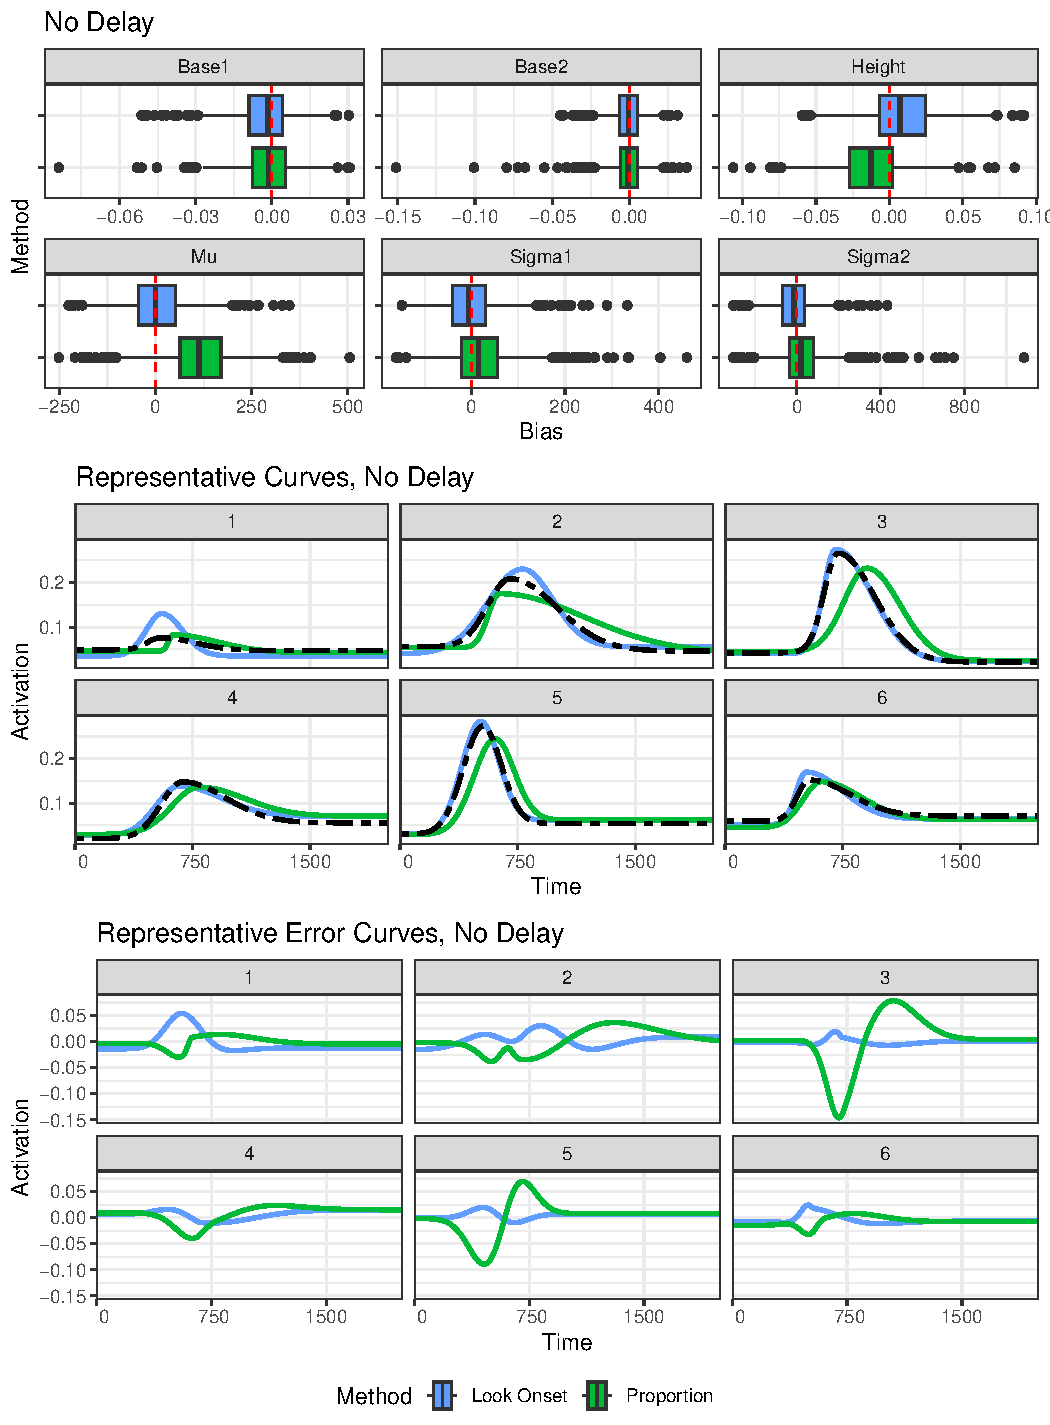
\includegraphics[width=0.9\textwidth]{dg_rep_and_diff_no_delay.pdf}
\caption{Summary of simulation results in the recovery of subject-specific curves generated by the asymmetric Gaussian with no oculomotor delay}
\label{fig:dg_rep_curves_no_delay}
\end{figure}

\begin{figure}[H]
\centering
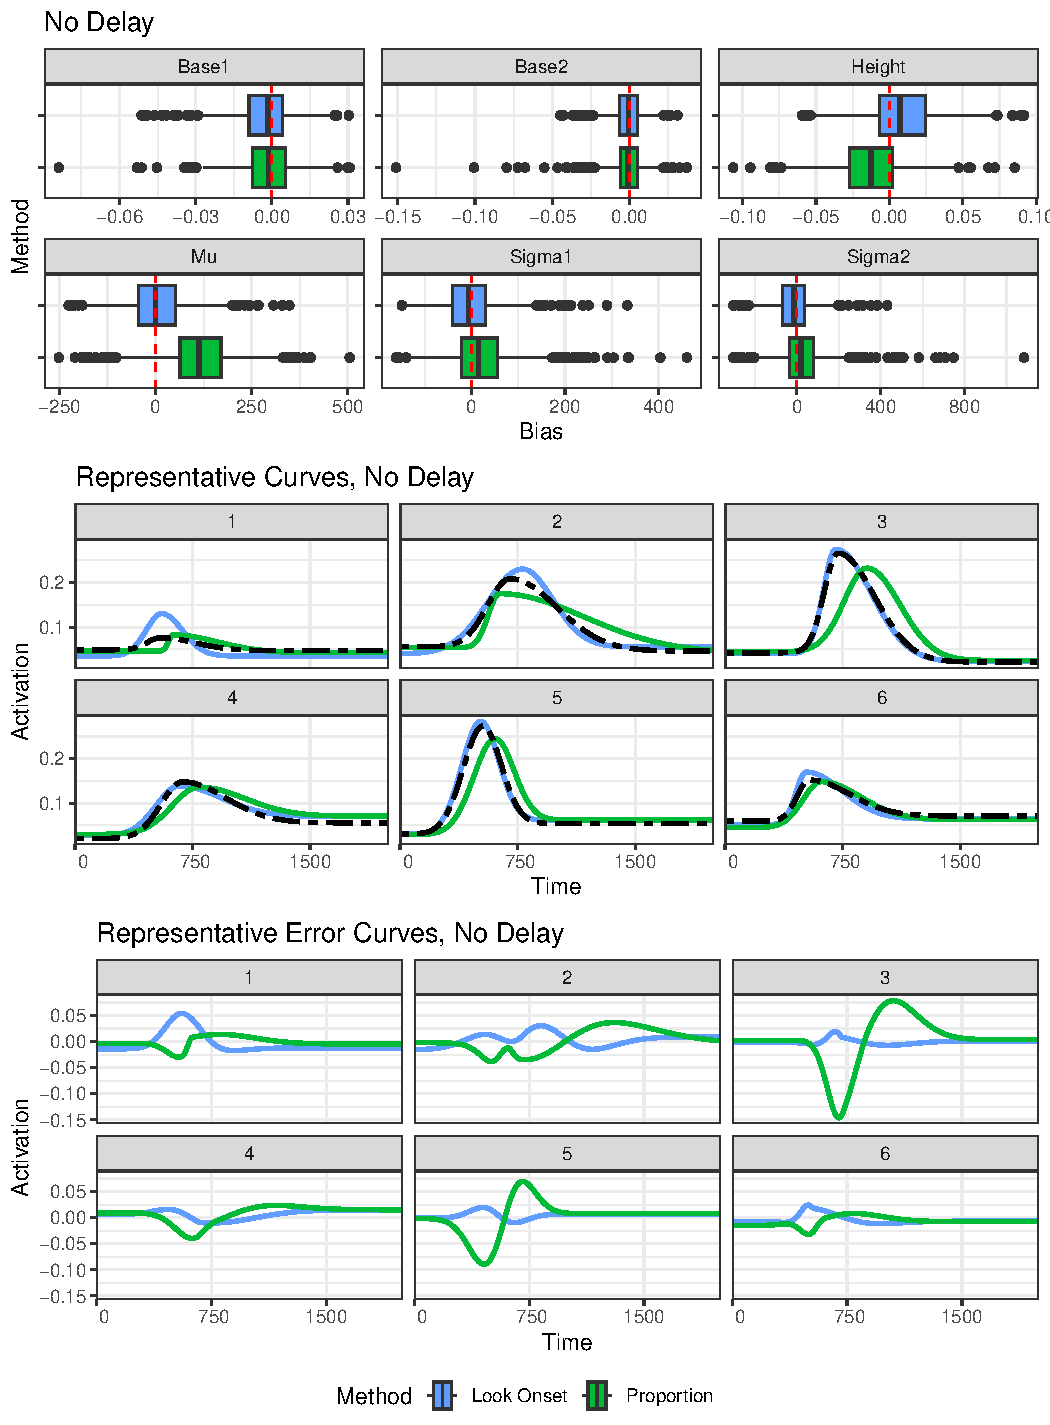
\includegraphics[width=0.9\textwidth]{dg_rep_and_diff_no_delay.pdf}
\caption{Summary of simulation results in the recovery of subject-specific curves generated by the asymmetric Gaussian with normally distributed oculomotor delay}
\label{fig:dg_rep_curves_normal_delay}
\end{figure}


\begin{figure}[H]
\centering
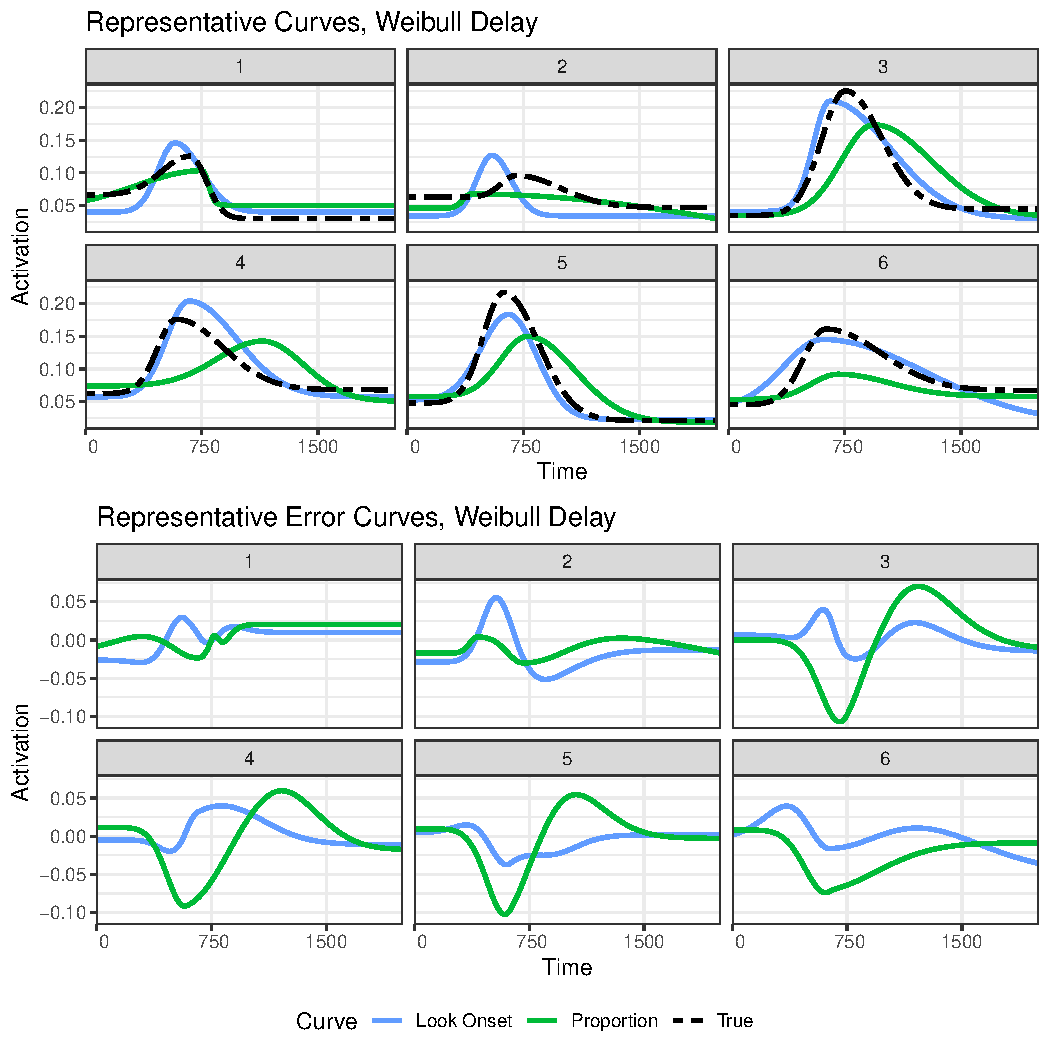
\includegraphics[width=0.9\textwidth]{dg_rep_and_diff_weibull_delay.pdf}
\caption{Summary of simulation results in the recovery of subject-specific curves generated by the asymmetric Gaussian with Weibull distributed oculomotor delay}
\label{fig:dg_rep_curves_weibull_delay}
\end{figure}




\begin{table}[H]
\centering
\begin{tabular}{llrrr}
  \hline
Curve & Delay & 1st Qu. & Median & 3rd Qu. \\ 
  \hline
Look Onset & No Delay & 0.22 & 0.36 & 0.63 \\ 
  Look Onset & Normal Delay & 0.38 & 0.70 & 1.15 \\ 
  Look Onset & Weibull Delay & 0.52 & 0.84 & 1.39 \\ 
  Proportion & No Delay & 0.75 & 1.29 & 2.08 \\ 
  Proportion & Normal Delay & 1.38 & 2.44 & 3.96 \\ 
  Proportion & Weibull Delay & 1.00 & 1.98 & 3.43 \\ 
   \hline
\end{tabular}
\caption{Median integrated squared error for recovery of individual curves generated with asymmetric Gaussian}
\label{tab:dg_mise_sims}
\end{table}

\subsection{$R^2$ for Recovery of Individual Curves}

Here, we provide an alternative summary of the recovery of subject specific curves fit with both the logistic and asymmetric Gauss. 


\subsubsection{Logistic}

\begin{table}[H]
\centering
\begin{tabular}{llrrr}
  \hline
Curve & Delay & 1st Qu. & Median & 3rd Qu. \\ 
  \hline
Look Onset & No Delay & 1.00 & 1.00 & 1.00 \\ 
  Look Onset & Normal Delay & 0.99 & 1.00 & 1.00 \\ 
  Look Onset & Weibull Delay & 0.98 & 0.99 & 0.99 \\ 
  Proportion & No Delay & 0.92 & 0.94 & 0.95 \\ 
  Proportion & Normal Delay & 0.80 & 0.83 & 0.86 \\ 
  Proportion & Weibull Delay & 0.80 & 0.86 & 0.91 \\ 
   \hline
\end{tabular}
\caption{$R^2$ for Logistic}
\label{tab:r2_logistic_sims}
\end{table}

\subsubsection{Asymmetric Gaussian}

\begin{table}[H]
\centering
\begin{tabular}{llrrr}
  \hline
Curve & Delay & 1st Qu. & Median & 3rd Qu. \\ 
  \hline
Look Onset & No Delay & 0.80 & 0.91 & 0.95 \\ 
  Look Onset & Normal Delay & 0.63 & 0.82 & 0.91 \\ 
  Look Onset & Weibull Delay & 0.57 & 0.77 & 0.87 \\ 
  Proportion & No Delay & 0.48 & 0.65 & 0.75 \\ 
  Proportion & Normal Delay & 0.10 & 0.33 & 0.52 \\ 
  Proportion & Weibull Delay & 0.20 & 0.46 & 0.64 \\ 
   \hline
\end{tabular}
\caption{$R^2$ for Asymmetric Gaussian}
\label{tab:r2_dg_sims}
\end{table}






